% This is LLNCS.DEM the demonstration file of
% the LaTeX macro package from Springer-Verlag
% for Lecture Notes in Computer Science,
% version 2.4 for LaTeX2e as of 16. April 2010
%
\documentclass{llncs}
%
%\usepackage{makeidx}  % allows for indexgeneration
%
\usepackage{paralist}
\usepackage{mathpartir}
\usepackage{comment}
\usepackage{amssymb}
\usepackage{amsfonts}
\usepackage{graphicx}
\usepackage{color}
\usepackage{multirow}
\usepackage{amsmath}
\usepackage{cite}
\usepackage{mathtools}

%% Commands For the syntax EBNF
\newcommand{\cfgnt}[1]{\emph{#1}}
\newcommand{\cfgq}[1]{\texttt{#1}}
\newcommand{\cfgt}[1]{\textbf{#1}}
\newcommand{\cfglhs}[1]{\cfgnt{#1} & $::=$}
\newcommand{\cfgrule}[2]{\cfglhs{#1} & #2 \\}
\newcommand{\cfgor}{\textbar\ }
\newcommand{\cfgstart}{\begin{tabular}{r@{\hspace{1mm}}r@{\hspace{2mm}}l}}
\newcommand{\cfgend}{\end{tabular}}
\newcommand{\cfgline}[1]{ ~ && #1 \\ }
\newcommand{\cfglinetab}[1]{ ~ && \hspace{1cm} #1 \\ }
\newcommand{\cfgorline}[1]{ ~ & \cfgor & #1 \\ }
\newcommand{\lp}{\cfgq{(}}
\newcommand{\lb}{\cfgq{[}}
\newcommand{\rp}{\cfgq{)}}
\newcommand{\rb}{\cfgq{]}}
\newcommand{\hsp}[0]{\hspace{1mm}}


\newcommand{\figref}[1]{Figure~\ref{#1}}
\newcommand{\secref}[1]{Section~\ref{#1}}
\newcommand{\thref}[1]{Theorem~\ref{#1}}
\newcommand{\lemref}[1]{Lemma~\ref{#1}}
\newcommand{\defref}[1]{Definition~\ref{#1}}
\newcommand{\appref}[1]{Appendix~\ref{#1}}

\newcommand{\sym}{\ensuremath{\varsigma}}
\newcommand{\gse}{\ensuremath{g}}
\newcommand{\rsym}{\ensuremath{\rightarrow_\sym}}
\newcommand{\rssym}{\ensuremath{\leadsto_\sym}}
\newcommand{\rgse}{\ensuremath{\rightarrow_\gse}}
\newcommand{\rsgse}{\ensuremath{\leadsto_\gse}}
\newcommand{\rsum}{\ensuremath{\rightarrow_S}}
\newcommand{\rinit}{\ensuremath{\rightarrow_I}}
\newcommand{\com}{\ensuremath{J}}
\newcommand{\rcom}{\ensuremath{\rightarrow_\com}}
\newcommand{\defeq}{\vcentcolon \vcentcolon=}

\newcommand{\sjp}[1]{\textcolor{blue}{#1}}

\newcommand{\symtxt}{symbolic initialization}
\newcommand{\gsetxt}{GSE}
\newcommand{\dsetxt}{DSE}

\newcommand{\nsr}[1]{\textcolor{red}{#1}}


\begin{document}
%
\title{Exact Heap Summaries for Symbolic Execution}
%
\author{Benjamin Hillery\inst{1} \and 
        Eric Mercer\inst{1} \and 
        Neha Rungta\inst{2} \and 
        Suzette Person\inst{3}}
%
\institute{Brigham Young University, Provo UT, USA
\and
NASA Ames, Mountain View CA, USA
\and
University of Nebraska, Lincoln NE, USA
}

\maketitle              % typeset the title of the contribution

\begin{abstract}
A recent trend in the analysis of object-oriented programs is the
modeling of references as sets of guarded values, enabling multiple
heap shapes to be represented in a single state. A fundamental problem
with using these guarded value sets is the creation of test inputs for
programs accepting symbolic reference input parameters. Although
several solutions have been proposed, none have been proven to be
sound and complete with respect to the properties provable by
generalized symbolic execution (GSE). This work presents a method for
initializing reference inputs in a symbolic input heap using guarded
value sets that exactly preserves GSE semantics. A correctness proof
for the initialization scheme is provided, as well as the results of
an empirical evaluation of a proof-of-concept implementation. The
initialization technique can be used to ensure that guarded value set
based symbolic execution engines operate in a provably correct manner
with regards to symbolic references.


%A fundamental challenge of using symbolic execution for software analysis is the treatment of dynamically allocated data. Existing techniques either underapproximate the space of possible inputs or are computationally infeasible. For example, dynamic symbolic execution (DSE) handles symbolic dereferencing by substituting in a value from a valid concrete execution. Generalized symbolic execution (GSE) initiates a new search path for every possible aliasing configuration. This paper introduces a method for de-referencing and manipulating values in a true block-box symbolic input heap that overcomes the limitations of previous methods. The symbolic heap supports arbitrary recursive data structures and captures all possible heaps that follow a common control flow path. Computation of complex preconditions and postconditions is supported, as well as automatic generation of test inputs. An evaluation of a proof-of-concept implementation in the Java Pathfinder framework is presented to demonstrate the computational feasibility of the approach over several classical symbolic execution benchmarks.


\keywords{symbolic execution, symbolic references, constraint-based reasoning}
\end{abstract}

\section{Introduction}

% SymExe is cool because for reasons x,y, and z

In recent years symbolic execution has provided the basis for various
software testing and analysis techniques. Symbolic execution
systematically explores the program execution space using symbolic
input values, and for each explored path, computes constraints on the
symbolic inputs to create a \emph{ path condition}.  The path
conditions computed by symbolic execution characterize the observed
program execution behaviors and have been used as an enabling
technology for various applications, e.g., regression
analysis~\cite{backes:2012,Godefroid:SAS11,Person:FSE08,person:pldi2011,Ramos:2011,Yang:ISSTA12},
data structure repair~\cite{KhurshidETAL05RepairingStructurally},
dynamic discovery of
invariants~\cite{CsallnerETAL08DySy,Zhang:ISSTA14}, and
debugging~\cite{Ma:2011}.

%
A major reason that path conditions are so useful is that each one represents exactly the set of concrete program inputs that would result in a given execution path. For any given program, a concrete execution will follow the same path as a symbolic execution if and only if the concrete inputs satisfy the path condition. Furthermore, because path conditions are logical predicates, they allow precise reasoning over potentially unbounded sets of program inputs. 

Symbolic execution's reliance on path conditions is both it's greatest strength, and a significant challenge. Since the path condition must be encoded in the form of an SMT problem, symbolic execution is limited by the capabilities of the underlying constraint solver. If the solver does not include a theory for reasoning about a given program operation, then the symbolic execution cannot proceed. Thus, extending the capabilities of symbolic execution to reason about new theories is an area of active research. 

One area of research involves symbolic reasoning for referencing operations. Of primary interest is dereferencing symbolic input references. There have been many proposed solutions for reasoning about symbolic input references, however to date none of them has been able to do so in a manner that preserves symbolic execution's most desirable property, namely the ability to produce a path condition that exactly represents all possible inputs for a given execution path.

% A couple of symExe�s big problems are path explosion and references. 

%Two of the main challenges facing current symbolic execution techniques 
%are path explosion and programs accepting references as inputs~\cite{Qu:2011,Chen:2013}.
% The path explosion problem stems from the way that 
%symbolic execution explores a program execution on a per-path basis. For 
%those programs for which there is an exponential number of possible 
%program paths, symbolic execution can be extremely inefficient. 
%References are a problem because symbolic execution requires that the 
%program state be represented by predicates formulated in terms of the 
%program inputs. Formulating such predicates for referencing operations 
%over potentially unbounded inputs has until now remained an open 
%question. 


% You can solve dereferencing by concretization, but that�s incomplete. 
%Here is an example of why this stinks.
One possible way to cope with the reference problem is to use a technique 
known as dynamic symbolic execution (DSE). When a DSE tool encounters 
an operation that is beyond the capabilities of its associated constraint 
solvers, such as dereferencing a symbolic reference, it substitutes a valid 
concrete result in place of the symbolic expression. However, this process 
of concretization introduces approximation into the formerly exact path condition,
and may even cause the analysis to miss valid program behaviors. 

%\begin{figure}
%void example( container a,b,c,d,x,y){
%a.f = x;
%b.f = c;
%c.f = d;
%d.f = a;
%if(x.f == y.f.f)
%     abort();\\error!
%}
%\caption{completeness example}
%\label{fig:DSEtest}
%\end{figure}
%
%Consider the example in \ref{fig:DSEtest}. During DSE, both symbolic and 
%concrete executions occur in parallel. Suppose that for the first pass, the 
%concrete execution picks the following points-to relationships: $a\rightarrow 
%loc_a, b\rightarrow loc_b, c\rightarrow loc_c, d\rightarrow loc_d ,x
%\rightarrow loc_a,  y\rightarrow loc_b$. When the program reaches the if() 
%statement, symbolic dereferencing of x and y are required. In order to 
%dereference symbol x to get x.f, x is concretized to point to $loc_a$, and 
%symbol x from field f is returned. Dereferencing y to find y.f requires 
%concretizing y to point to $loc_b$, From there, dereferencing b.f gives us 
%the reference d as the final value for y.f.f . Assuming the �false" branch is 
%executed first, the branch condition (x.f != y.f.f) reduces to x!=d, which 
%evaluates to �true" and DSE proceeds until program termination.
%After following the false branch, DSE will attempt to follow the true branch, 
%but the branch condition x==d will evaluate to false, and so DSE will 
%attempt a second pass starting from the beginning with a modified path 
%condition. For the second pass, DSE adds x==d to the path condition from 
%the beginning, to try to get the �true� branch. This time, the concrete 
%execution will choose x to point to $loc_d$. When evaluating the branch 
%condition, x.f will evaluate to a. Since the value for y is unchanged, the read 
%from y.f.f evaluates to d. The branch condition reduces to a==d, which 
%evaluates to false, so the �true� branch cannot be followed. In this instance, 
%DSE will fail to find a path to the error condition. 

% You can model references by forking the system state, but that makes 
%path explosion worse.
An alternative to concretization is to construct the input heap in a lazy manner,
deferring materialization of objects on the concrete heap until they
are needed for the analysis to proceed. The materialization creates
additional non-deterministic choice points in the symbolic execution
tree by representing the feasible heap configurations as (i) null,
(ii) an instance of a new reference of a compatible class, and (iii)
an alias to a previously initialized symbolic reference.  Symbolic
execution then follows concrete program semantics for materialized
heap locations. Although this approach enables the analysis of heap
manipulating programs, a large number of feasible concrete heap
configurations are created. Since each configuration requires a separate
path, GSE induces a path explosion problem while at the 
same time splitting the symbolic input space and decreasing the 
utility of the path condition.

% You can solve path explosion by bounding the execution and rolling 
%everything into one big equation, but then you�re incomplete. Here is an 
%example why that stinks.
%-maybe point out that finding the right bounds is a hard problem
One solution to the path explosion problem is to model the input heap as a 
predicate over a bounded set of locations. This allows the analysis to 
maintain a single representation for a set of possible heap configurations 
on each execution path, without case splitting for dereferencing operations. 
However, by placing an arbitrary bounds on the size of the input heap, neither
the path condition, nor the analysis performed by these techniques is complete.

% This paper introduces a technique that is, to the best knowledge of the 
%authors, the first sound and complete heap for SymEXE
This paper introduces a technique for modeling references and their 
associated operations that is both sound and complete\footnote{with 
respect to the properties provable by symbolic execution}, and models all 
possible heap configurations along a given execution path. To the 
knowledge of the authors, it is the first technique to do so. 

THIS NEXT BIT NEEDS SOME WORK, STILL:

% Creating this technique required the following key insights:
These advances were enabled by the following key insights: 

First, that a complete analysis requires an unconstrained input heap. 
However, it is unclear from prior work how this might be accomplished.

Second, that GSE techniques needlessly split during dereferencing 
operations. If GSE was performing a concretization, as in DSE, then case 
splitting makes more sense. However, lazy initialization is not a 
concretization, and is in fact only a partitioning of the input space. 

Third, that we can combine lazy initialization with a compositional heap 
abstraction to form constraints on a potentially unbounded input heap.


% This paper makes the following contributions.


\noindent{This paper makes the following contributions:}

\begin{compactdesc}

\item\textbf{-} The first sound and complete system for reasoning symbolically about the 
set of input heaps along any valid program path. 

\item\textbf{-} A bisimulation proof establishing the soundness and 
completeness of the heap summary approach with respect to
properties provable by GSE.

\item\textbf{-} A proof-of-concept implementation and empirical study 
demonstrating the scalability of the summary heap approach
compared to other GSE approaches.

\end{compactdesc}


%Initial work on symbolic execution largely focused on checking
%properties of programs with primitive
%types~\cite{clarke76TSE,King:76}.  With the advent of object-oriented
%languages, recent work has generalized the core ideas of symbolic
%execution to enable analysis of programs containing complex data
%structures with unbounded domains, i.e., data stored on the
%heap~\cite{Kiasan06,Kiasan07,GSE03}.  These \emph{Generalized 
%Symbolic
%  Execution} (GSE) techniques construct the heap in a lazy manner,..

%The goal of this work is to mitigate the path explosion problem in GSE
%by grouping multiple heaps together and only partitioning the heaps at
%points of divergence in the control flow graph. Our inspiration is
%found in the domain of static analysis that uses sets of constraints
%over heap locations to encode multiple heaps in a single
%representation. These sets, sometimes known as \emph{value sets} or
%\emph{value summaries}, allow multiple heaps to be represented
%simultaneously with a higher degree of precision than afforded by
%traditional techniques for shape analysis. Some of these previous
%attempts, however, are unable to handle aliasing in heaps due to a
%recursive definition of objects~\cite{Xie:2005}, while others require
%a set of heaps as input and are unable to initialize heaps
%on-the-fly~\cite{Dillig:2011,Tillmann:2008}.  As is typical in static
%analysis, over approximation of the heap representations alleviates
%some of these limitations but often leads to infeasible heaps. Also,
%most static analysis techniques for heap updates require a rewrite of
%the constraint system making it prohibitive for use in the context of
%symbolic execution.

%In this work, to effectively represent multiple heaps simultaneously
%in the context of symbolic execution, we define a novel heap
%representation and an algorithm to initialize and update the heap
%on-the-fly. In essence, our summary heap approach supports aliasing,
%does not require constraint rewriting on heap updates, and reduces
%non-determinism in the search space during symbolic execution.
%
%We represent the heap as a bipartite graph consisting of references
%and locations. Each reference is able to point to multiple locations,
%where each edge is predicated on constraints over aliasing between
%references. Each location points to a single reference for a given
%field. The use of a bipartite graph affords two key advantages: (i) it
%allows for a non-recursive definition of objects which enables us to
%support aliasing, and (ii) it does not introduce auxiliary variables
%or require rewriting of non-local constraints during updates to the
%heap.
%
%The summary heap algorithm defines how the bipartite graph is updated
%during lazy initialization. Unlike GSE, however, the summary heap
%algorithm introduces non-determinism in the search only at points of
%divergence in the control flow graph. These points of non-determinism
%are at field accesses that lead to null-pointer exceptions and at
%comparisons of references. The former represents a divergence due to
%exceptional control flow while the latter is due to program structure.
%The combination of the heap representation and the summary heap
%algorithm enables us to improve the efficiency of symbolic execution
%of heap manipulating programs over state-of-the-art techniques.
%
%The summary heap algorithm is sound and complete with respect to
%properties that are provable using GSE. This proof is accomplished by
%showing the existence of a bisimulation between states in GSE and
%states in the summary heap algorithm.  A preliminary implementation in
%Java Pathfinder (JPF) shows that in general, the heap summary
%algorithm improves over other state-of-the-art techniques, and in some
%instances, the improvement is remarkable: two-orders of magnitude
%reduction in running time. More importantly though, the heap summary
%enables the initialization of larger more complex heaps than
%previously possible as shown in our results.


\section{A Symbolic Heap}
A \emph{symbolic heap} is a tuple
$(\cfgnt{L}\ \cfgnt{R}\ \phi\ \eta)$, where the~\emph{location map}
$\cfgnt{L}$,~\emph{reference map} $\cfgnt{R}$, and~\emph{environment}
$\eta$ are partial functions, and the~\emph{path condition} $\phi$ is
a predicate over the program variables. Given reference $r$,
$\cfgnt{L}(r) = \{(\phi\ \cfgnt{l})\ ...\}$ is the guarded value set
in the heap associated with $r$. The constraint associated with each
location is a guard representing the conditions under which the
associated reference maps to the given location. By definition, any
location appears at most once in any given value set. Unions of value
sets containing the same location are resolved by forming a
disjunction of the constraints from each set. $\cfgnt{R}(\cfgnt{l},
\cfgnt{f}) = \cfgnt{r}$ is the reference associated with the given
location-field pair in the heap. 

\begin{figure}[t]
\begin{center}
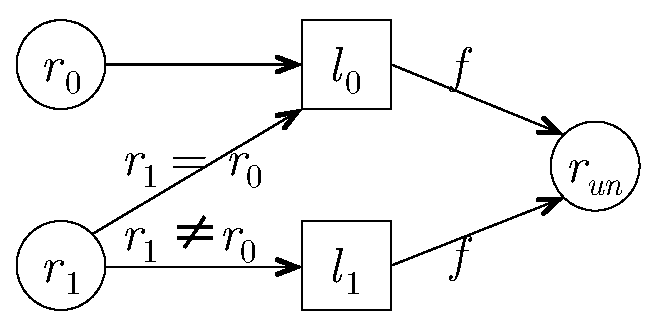
\includegraphics[scale=0.5]{../figs/simple_heap_scratch.pdf}
\end{center}
\caption{Example Symbolic Heap}
\label{fig:exampleHeap}
\end{figure}

Conceptually, the symbolic heap may be thought of as a bipartite
graph. \figref{fig:exampleHeap} shows an example symbolic heap
graph. References are represented by circles and locations are
represented by squares. Arrows leaving references correspond to the
guarded value sets returned by the $\cfgnt{L}$ function, and arrows
leaving the squares correspond to the $\cfgnt{R}$ function. The
reference $\cfgnt{r}_1$ has has two members in it guarded value set,
so the location pointed to by $\cfgnt{r}_1$ depends on its aliasing
relationship to $\cfgnt{r}_0$.

The reference $\cfgnt{r}_\mathit{un}$ is a special reference to
indicate something that has yet to be initialized. In general,every
symbolic heap contains two special locations, null
($\cfgnt{l}_\mathit{null}$), and uninitialized
($\cfgnt{l}_\mathit{un}$), with corresponding references
$\cfgnt{r}_\mathit{null}$ and $\cfgnt{r}_\mathit{un}$ where
$\cfgnt{L}(\cfgnt{r}_\mathit{null}) =
\{(\cfgt{true}\ \cfgnt{l}_\mathit{null})\}$ and
$\cfgnt{L}(\cfgnt{r}_\mathit{un}) =
\{(\cfgt{true}\ \cfgnt{l}_\mathit{un})\}$.

For well-formed symbolic heaps, a reference in $(\cfgnt{L}\ \cfgnt{R})$ cannot point to multiple locations simultaneously: 
$
\forall \cfgnt{r} \in \cfgnt{L}^\leftarrow\ (\forall (\phi\ \cfgnt{l}),(\phi^\prime\ \cfgnt{l}^\prime) \in \cfgnt{L}(r)\ (
(\cfgnt{l} \neq \cfgnt{l}^\prime \vee \phi \neq \phi^\prime) \Rightarrow (\phi \wedge \phi^\prime = \cfgt{false}))
$
where $\cfgnt{L}^\leftarrow$ is the pre-image of $\cfgnt{L}$. Also, for a well-formed heap, all locations associated with a reference have the same type:
$\forall \cfgnt{r} \in \cfgnt{L}^\leftarrow\ (\forall (\phi\ \cfgnt{l}),(\phi^\prime\ \cfgnt{l}^\prime) \in \cfgnt{L}(r)\ (
(\mathrm{Type}\lp\cfgnt{l}\rp = \mathrm{Type}\lp\cfgnt{l}^\prime\rp)))$

\section{Operational Semantics}
This paper defines symbolic initialization using
a small-step operational semantics in the context of a syntactic machine with a CESK architecture~\cite{Felleisen:1992, saints-MS}. The
surface (input) syntax and machine (state) syntax (which omits the symbolic heap definition previously given and the environment) are shown
in~\figref{fig:syntax}. Terminals are in bold face while non-terminals
are italicized. Ellipses indicate zero or more repetitions. Tuples
omit the commas for compactness.

\begin{figure}
\begin{center}
\cfgstart
\cfgrule{P}{\lp $\mu$ \lp \cfgnt{C} \cfgnt{m}\rp\rp}
\cfgrule{$\mu$}{(\cfgnt{CL} ...)}
\cfgrule{T}{\cfgt{bool} \cfgor \cfgnt{C}}
\cfgrule{CL}{\lp\cfgt{class} \cfgnt{C} \lp\lb\cfgnt{T} \cfgnt{f}\rb ...\rp \lp\cfgnt{M} ...\rp}
\cfgrule{M}{\lp\cfgnt{T} \cfgnt{m} \lb\cfgnt{T} \cfgnt{x}\rb\  e\rp}
\cfgrule{e}{\cfgnt{x}
\cfgor{\lp\cfgt{new} \cfgnt{C}\rp}
\cfgor{\lp\cfgnt{e} \cfgt{\$} \cfgnt{f}\rp}
\cfgor{\lp\cfgnt{x} \cfgt{\$} \cfgnt{f} \cfgt{:=} \cfgnt{e}\rp}
\cfgor{\lp\cfgnt{e} \cfgt{=} \cfgnt{e}\rp}}
\cfgorline{\lp\cfgt{if} \cfgnt{e} \cfgnt{e} \cfgt{else} \cfgnt{e}\rp 
\cfgor {\lp\cfgt{var} \cfgnt{T} \cfgnt{x} \cfgt{:=} \cfgnt{e} \cfgt{in} \cfgnt{e}\rp}
\cfgor {\lp\cfgnt{e} \cfgt{@} \cfgnt{m} \cfgnt{e} \rp}}
\cfgorline{\lp\cfgnt{x} \cfgt{:=} \cfgnt{e}\rp
\cfgor{\lp\cfgt{begin} \cfgnt{e} ...\rp}
\cfgor{\cfgnt{v}}}
\cfgrule{x}{\cfgt{this} \cfgor \cfgnt{id}}
\cfgrule{f,m,C}{\cfgnt{id}}
%\cfgrule{m}{\cfgnt{id}}
%\cfgrule{C}{\cfgnt{id}}
\cfgrule{v}{\cfgnt{r} \cfgor \cfgt{null} \cfgor \cfgt{true} \cfgor \cfgt{false} \cfgor \cfgt{error}}
\cfgrule{r}{\cfgt{number}}
\cfgrule{id}{\cfgt{variable-not-otherwise-mentioned}}
\cfgend
\end{center}
\caption{The Javalite surface syntax.}
\label{fig:surface-syntax}
\end{figure}

\begin{figure}
\begin{center}
\cfgstart
\cfgrule{e}{\lp ... \cfgor \lp \cfgnt{v} \cfgt{@} \cfgnt{m} \cfgnt{v} \rp\rp}
%\cfgrule{object}{ (\cfgnt{C} [ \cfgnt{f} \cfgnt{loc} ] ...) }
%\cfgrule{hv}{ (\cfgnt{v} \cfgnt{object})}
\cfgrule{$\phi$}{\cfgnt{constraint}}
\cfgrule{l}{\cfgt{number}}
%\cfgrule{h}{(\cfgnt{mt}\ (\cfgnt{h}\ [\cfgnt{loc} $\rightarrow$ \cfgnt{hv}]) )}
\cfgrule{$\eta$}{(\cfgnt{mt}\ ($\eta$ [\cfgnt{x} $\rightarrow$ \cfgnt{loc}]))}
\cfgrule{s}{\lp$\mu$ \cfgnt{L} \cfgnt{R} \cfgnt{g} $\eta$ \cfgnt{e} \cfgnt{k}\rp}
\cfgrule{k}{\cfgt{end}}
\cfgorline{\lp \cfgt{*} \cfgt{\$} \cfgnt{f} $\rightarrow$ \cfgnt{k}\rp}
\cfgorline{\lp \cfgt{*} \cfgt{@} \cfgnt{m} \lp \cfgnt{e} ... \rp $\rightarrow$ \cfgnt{k} \rp}
\cfgorline{\lp \cfgnt{v} \cfgt{@} \cfgnt{m} \cfgnt{v} \cfgt{*} \lp \cfgnt{e} ... \rp $\rightarrow$ \cfgnt{k} \rp}
\cfgorline{\lp \cfgt{*} \cfgt{=} \cfgnt{e} $\rightarrow$ \cfgnt{k}\rp}
\cfgorline{\lp \cfgt{v} \cfgt{=} \cfgnt{*} $\rightarrow$ \cfgnt{k}\rp}
\cfgorline{\lp \cfgt{x} \cfgt{:=} \cfgnt{*} $\rightarrow$ \cfgnt{k}\rp}
\cfgorline{\lp \cfgt{x} \cfgt{\$} \cfgnt{f}  \cfgt{:=} \cfgnt{*} $\rightarrow$ \cfgnt{k}\rp}
\cfgorline{\lp \cfgt{if} \cfgnt{*} \cfgnt{e} \cfgt{else} \cfgnt{e} $\rightarrow$ \cfgnt{k} \rp}
\cfgorline{\lp\cfgt{var} \cfgnt{T} \cfgnt{x} \cfgt{:=} \cfgnt{*} \cfgt{in} \cfgnt{e}  $\rightarrow$ \cfgnt{k} \rp}
\cfgorline{\lp\cfgt{begin}  \cfgnt{*} \lp \cfgnt{e} ...\rp $\rightarrow$ \cfgnt{k} \rp}
\cfgorline{\lp\cfgt{pop} $\eta$ \cfgnt{k}\rp}
\cfgend
\end{center}
\caption{The machine syntax for Javalite.}
\label{fig:machine-syntax}
\end{figure}

\begin{figure}[t]
\begin{center}
\begin{tabular}{c}
\scalebox{0.9}{\usebox{\boxSurface}} \\
(a) \\\\
\scalebox{0.9}{\usebox{\boxMachine}} \\
(b)
\end{tabular}
\end{center}
\caption{ (a) The surface syntax. (b) The machine syntax with $\bowtie\ \in \{\wedge,\vee,\Rightarrow\}$.}
\label{fig:syntax}
\end{figure}

A program, $\cfgnt{P}$, is a registry of classes, $\mu$, with
a tuple indicating a class, $\cfgnt{C}$, and a method, $\cfgnt{m}$,
where execution starts. For simplicity in presentation, booleans are the only primitive type, 
classes have only non-primitive fields, and methods have a single
parameter. Expressions, $\cfgnt{e}$, include statements, and they use
'$\cfgt{:=}$' to indicate assignment and '$\cfgt{=}$' to indicate
comparison.  The dot-operator for field access is replaced by
'$\cfgt{\$}$', and the dot-operator for method invocation is replaced
by '$\cfgt{@}$'. There is no
explicit return statement; rather, the value of the last expression is
used as the return value. A variable is always indicated by \cfgnt{x}
and a value by \cfgnt{v}. A value can be a reference in the heap,
$\cfgnt{r}$, or any of the special values shown
in~\figref{fig:syntax}(a).  Only type correct programs are given as
input to the machine.


The machine state $\cfgnt{s}$ includes the program
registry $\mu$, the symbolic heap, the global path constraint, the environment $\eta$, the current expression (i.e., program), and the continuation $\cfgnt{k}$. The registry never changes so it is
omitted from the state tuple in the rest of the presentation. The environment is a partial function so $\eta(\cfgnt{x}) = \cfgnt{r}$ is the reference
$\cfgnt{r}$ associated with variable $\cfgnt{x}$. The notation
$\eta^\prime = \eta[\cfgnt{x} \mapsto \cfgnt{v}]$ defines a new
partial function $\eta^\prime$ that is the same as $\eta$ except that
the variable $\cfgnt{x}$ now maps to $\cfgnt{v}$. This notation is used with symbolic heaps as well. 

The continuation
$\cfgnt{k}$ indicates with the symbol $\cfgnt{*}$ where the expression $\cfgnt{e}$ came from, stores
temporary computation, and keeps track of the next continuation. For
example, the continuation $\lp\cfgt{*}\ \cfgt{\$}\ \cfgnt{f}
\rightarrow \cfgnt{k}\rp$ indicates that the machine is evaluating the
expression for the object reference on which the field $\cfgnt{f}$ is
going to be accessed. Once the field access is complete, the machine
continues with $\cfgnt{k}$.  

Given an input program $\lp\mu\ \lp\cfgnt{C}\ \cfgnt{m}\rp\rp$, the expression for the initial machine state is
$$
\begin{array}{l}
\lp\mu 
\ \cfgnt{L}[\cfgnt{r}_\mathit{null} \mapsto \{\lp\cfgt{true}\ \cfgnt{l}_\mathit{null})\}\rp] 
           [\cfgnt{r}_\mathit{un} \mapsto \{\lp\cfgt{true}\ \cfgnt{l}_\mathit{un}\rp\}] \\
\ \cfgnt{R}
\ \cfgt{true}\ \eta\  \lp\lp\cfgt{new}\ \cfgnt{C}\rp\ \cfgt{@}\ \cfgnt{m}\ \cfgt{true}\rp\rp\ \cfgt{end}\rp
\end{array}
$$
The semantics are expressed as
rewrites on strings using pattern matching. 
Consider the rewrite rule
for the beginning of a field access instruction:
$$
\mprset{flushleft}
	\inferrule[Field Access(eval)]{}{
      \lp \cfgnt{L}\ \cfgnt{R}\ \phi\ \eta\ \lp \cfgnt{e}\ \cfgt{\$}\ \cfgnt{f}\rp \ \cfgnt{k}\rp  \rcom 
      \lp \cfgnt{L}\ \cfgnt{R}\ \phi\ \eta\ \cfgnt{e}\ \lp \cfgt{*}\ \cfgt{\$}\ \cfgnt{f} \rightarrow \cfgnt{k}\rp \rp 
	}
$$
If the string representing the current state matches the left side, then it
creates the new string on the right. In this example, the new string
on the right is now evaluating the expression $\cfgnt{e}$ in the field
access, and it includes the continuation indicating that it still
needs to complete the actual field access once the expression is
evaluated.
%
%Other more complex rules, such as one to create a new instance of a
%class, define constraints on the rewrites and more complex
%transformations on the heap.
%$$
%\mprset{flushleft}
%	\inferrule[New]{
%      \cfgnt{r} = \mathrm{stack}_r\lp \rp\\
%      l = \mathrm{fresh}_l\lp \cfgnt{C}\rp\\\\
%      \cfgnt{R}^\prime = \cfgnt{R}[\forall \cfgnt{f} \in \mathit{fields}\lp \mathrm{C}\rp \ \lp \lp l\ \cfgnt{f}\rp  \mapsto \cfgnt{r}_\mathit{null} \rp ] \\\\
%      \cfgnt{L}^\prime = \cfgnt{L}[\cfgnt{r} \mapsto \{\lp \cfgt{true}\ l\rp \}]
%    }{
%      \lp \cfgnt{L}\ \cfgnt{R}\ \phi\ \eta\ \lp \cfgt{new}\ \cfgnt{C}\rp \ \cfgnt{k}\rp  \rcom
%      \lp \cfgnt{L}^\prime\ \cfgnt{R}^\prime\ \phi\ \eta\ \cfgnt{r}\ \cfgnt{k}\rp 
%	}
%$$ In this rule, when the string matches the new-expression, it is
%        rewritten to use a new heap location where all of the fields
%        for the new object point to $\cfgnt{r}_\mathit{null}$ and the
%        location map points a new stack reference to that new object.
%        New heap locations returned from $\mathrm{fresh}_l$ are monotonically
%        increasing.
%        Also note that references for objects from the new-expression are
%        auxiliary literals, so they do not appear in any constraint in
%        the symbolic heap as an aliasing option. 
%        
% \begin{figure*}[t]
\begin{center}
\mprset{flushleft}
\begin{mathpar}
	\inferrule[Variable lookup]{}{
      \lp \cfgnt{L}\ \cfgnt{R}\ \phi\ \eta\ \cfgnt{x}\ \cfgnt{k}\rp  \rcom \\\\
      \lp \cfgnt{L}\ \cfgnt{R}\ \phi\ \eta\ \eta\lp \cfgnt{x}\rp \ \cfgnt{k}\rp 
	}
\and
	\inferrule[New]{
      \cfgnt{r} = \mathrm{stack}_r\lp \rp\\
      l = \mathrm{fresh}_l\lp \cfgnt{C}\rp\\\\
      \cfgnt{R}^\prime = \cfgnt{R}[\forall \cfgnt{f} \in \mathit{fields}\lp \mathrm{C}\rp \ \lp \lp l\ \cfgnt{f}\rp  \mapsto \cfgnt{r}_\mathit{null} \rp ] \\\\
      \cfgnt{L}^\prime = \cfgnt{L}[\cfgnt{r} \mapsto \{\lp \cfgt{true}\ l\rp \}]
    }{
      \lp \cfgnt{L}\ \cfgnt{R}\ \phi\ \eta\ \lp \cfgt{new}\ \cfgnt{C}\rp \ \cfgnt{k}\rp  \rcom
      \lp \cfgnt{L}^\prime\ \cfgnt{R}^\prime\ \phi\ \eta\ \cfgnt{r}\ \cfgnt{k}\rp 
	}
\and
	\inferrule[Field Access(eval)]{}{
      \lp \cfgnt{L}\ \cfgnt{R}\ \phi\ \eta\ \lp \cfgnt{e}\ \cfgt{\$}\ \cfgnt{f}\rp \ \cfgnt{k}\rp  \rcom \\\\
      \lp \cfgnt{L}\ \cfgnt{R}\ \phi\ \eta\ \cfgnt{e}\ \lp \cfgt{*}\ \cfgt{\$}\ \cfgnt{f} \rightarrow \cfgnt{k}\rp \rp 
	}
\and
	\inferrule[Field Write (eval)]{}{
       \lp \cfgnt{L}\ \cfgnt{R}\ \phi\ \eta\ \lp \cfgnt{x}\ \cfgt{\$}\ \cfgnt{f}\ \cfgt{:=}\ \cfgnt{e}\rp \ \cfgnt{k}\rp  \rcom \\\\
       \lp \cfgnt{L}\ \cfgnt{R}\ \phi\ \eta\ \cfgnt{e}\ \lp \cfgnt{x}\ \cfgt{\$}\ \cfgnt{f}\ \cfgt{:=}\ \cfgt{*}\ \rightarrow\ \cfgnt{k}\rp \rp 
	}
\and
    \inferrule[Equals (l-operand eval)]{}{
      \lp \cfgnt{L}\ \cfgnt{R}\ \phi\ \eta\ \lp \cfgnt{e}_0\ \cfgt{=}\ \cfgnt{e}\rp  \ \cfgnt{k}\rp  \rcom \\\\
      \lp \cfgnt{L}\ \cfgnt{R}\ \phi\ \eta\ \cfgnt{e}_0\ \lp \cfgt{*}\ \cfgt{=}\; \cfgnt{e} \rightarrow \cfgnt{k}\rp \rp 
    }
\and
    \inferrule[Equals (r-operand eval)]{}{
    \lp \cfgnt{L}\ \cfgnt{R}\ \phi\ \eta\ \cfgnt{v}\ \lp \cfgt{*}\; \cfgt{=}\; \cfgnt{e} \rightarrow \cfgnt{k}\rp \rp  \rcom \\\\
    \lp \cfgnt{L}\ \cfgnt{R}\ \phi\ \eta\ \cfgnt{e}\ \lp \cfgnt{v}\; \cfgt{=}\; \cfgt{*} \rightarrow \cfgnt{k}\rp \rp 
    }
\and
    \inferrule[Equals (bool)]{
    \cfgnt{v}_0 \in \{\cfgt{true}, \cfgt{false}\} \\
    \cfgnt{v}_1 \in \{\cfgt{true}, \cfgt{false}\} \\\\
    \cfgnt{v}_r = \mathrm{eq?}\lp \cfgnt{v}_0, \cfgnt{v}_1\rp}{
    \lp \cfgnt{L}\ \cfgnt{R}\ \phi\ \eta\ \cfgnt{v}_0\ \lp \cfgnt{v}_1\; \cfgt{=}\; \cfgt{*} \rightarrow \cfgnt{k}\rp \rp  \rcom \\\\
    \lp \cfgnt{L}\ \cfgnt{R}\ \phi\ \eta\ \cfgnt{v}_r\ \cfgnt{k}\rp 
    }
\and
    \inferrule[If-then-else (eval)]{}{
      \lp \cfgnt{L}\ \cfgnt{R}\ \phi\ \eta\ \lp \cfgt{if}\ \cfgnt{e}_0\ \cfgnt{e}_1\ \cfgt{else}\ \cfgnt{e}_2\rp \ \cfgnt{k}\rp  \rcom \\\\
      \lp \cfgnt{L}\ \cfgnt{R}\ \phi\ \eta\ \cfgnt{e}_0\ \lp \cfgt{if}\ \cfgt{*}\ \cfgnt{e}_1\ \cfgt{else}\ \cfgnt{e}_2\rp  \rightarrow \cfgnt{k}\rp 
	}
\and
	\inferrule[If-then-else (true) ]{}{
       \lp \cfgnt{L}\ \cfgnt{R}\ \phi\ \eta\ \cfgt{true}\ \lp \cfgt{if}\ \cfgt{*}\ \cfgnt{e}_1\ \cfgt{else}\ \cfgnt{e}_2\rp  \rcom \cfgnt{k}\rp  \rightarrow \\\\
       \lp \cfgnt{L}\ \cfgnt{R}\ \phi\ \eta\ \cfgnt{e}_1\  \cfgnt{k}\rp 
	}
\and
	\inferrule[If-then-else (false)]{}{
       \lp \cfgnt{L}\ \cfgnt{R}\ \phi\ \eta\ \cfgt{false}\ \lp \cfgt{if}\ \cfgt{*}\ \cfgnt{e}_1\ \cfgt{else}\ \cfgnt{e}_2\rp  \rcom \cfgnt{k}\rp  \rightarrow \\\\
       \lp \cfgnt{L}\ \cfgnt{R}\ \phi\ \eta\ \cfgnt{e}_2\  \cfgnt{k}\rp 
	}
\and
   \inferrule[Variable Declaration (eval)]{}{
    \lp \cfgnt{L}\ \cfgnt{R}\ \phi\ \eta\ \lp\cfgt{var}\ \cfgnt{T}\ \cfgnt{x}\ \cfgt{:=}\ \cfgnt{e}_0\ \cfgt{in}\ \cfgnt{e}_1\rp\ \cfgnt{k}\rp  \rcom \\\\
    \lp \cfgnt{L}\ \cfgnt{R}\ \phi\ \eta\ \cfgnt{e}_0\ \lp\cfgt{var}\ \cfgnt{T}\ \cfgnt{x}\ \cfgt{:=}\ \cfgt{*}\ \cfgt{in}\ \cfgnt{e}_1 \rightarrow \cfgnt{k}\rp\rp 
   }	
\and
   \inferrule[Variable Declaration]{}{
    \lp \cfgnt{L}\ \cfgnt{R}\ \phi\ \eta\ \cfgnt{v}\ \lp\cfgt{var}\ \cfgnt{T}\ \cfgnt{x}\ \cfgt{*}\ \cfgt{:=}\ \cfgt{in}\ \cfgnt{e}_1 \rightarrow \cfgnt{k}\rp\rp  \rcom \\\\
    \lp \cfgnt{L}\ \cfgnt{R}\ \phi\ \eta[x \mapsto \cfgnt{v}]\ \cfgnt{e}_1\ \lp \cfgt{pop}\ \eta\ \cfgnt{k}\rp \rp 
   }	
\and
   \inferrule[Method Invocation (object eval)]{}{
    \lp \cfgnt{L}\ \cfgnt{R}\ \phi\ \eta\ \lp\cfgnt{e}_0\ \cfgt{@}\ \cfgnt{m}\ \cfgnt{e}_1\rp\ \cfgnt{k}\rp  \rcom \\\\
    \lp \cfgnt{L}\ \cfgnt{R}\ \phi\ \eta\ \cfgnt{e}_0\ \lp \cfgt{*}\ \cfgt{@}\ \cfgnt{m}\ \cfgnt{e}_1\ \rightarrow \cfgnt{k}\rp \rp 
   }
\and
   \inferrule[Method Invocation (arg eval)]{}{
    \lp \cfgnt{L}\ \cfgnt{R}\ \phi\ \eta\ \cfgnt{v}_0\ \lp \cfgt{*}\ \cfgt{@}\ \cfgnt{m}\ \cfgnt{e}_1\ \rightarrow \cfgnt{k}\rp \rp  \rcom \\\\
    \lp \cfgnt{L}\ \cfgnt{R}\ \phi\ \eta\ \cfgnt{e}_1\ \lp \cfgnt{v}_0\ \cfgt{@}\ \cfgnt{m}\ \cfgt{*}\ \rightarrow \cfgnt{k}\rp \rp 
   }
\and
   \inferrule[Method Invocation]{
    \cfgnt{C} = \mathrm{type}\lp\cfgnt{r}\rp \\\\
    \lp\cfgnt{T}_o\ \cfgnt{m}\ \lb\cfgnt{T}_1\ \cfgnt{x}\rb\ \ \cfgnt{e}_m\rp = \mathrm{lookup}\lp \cfgnt{C},\cfgnt{m}\rp\\\\
    \eta_m = \eta[\cfgt{this} \mapsto \cfgnt{r}][\cfgnt{x} \mapsto \cfgnt{v}]}{
    \lp \cfgnt{L}\ \cfgnt{R}\ \phi\ \eta\ \cfgnt{v}\ \lp \cfgnt{r}\ \cfgt{@}\ \cfgnt{m}\ \cfgt{*}\ \rightarrow \cfgnt{k}\rp \rp  \rcom \\\\
    \lp \cfgnt{L}\ \cfgnt{R}\ \phi\ \eta_m\ \cfgnt{e}_m\ \lp \cfgt{pop}\ \eta\ \cfgnt{k}\rp \rp 
   }
\and
   \inferrule[Variable Assignment (eval)]{}{
    \lp \cfgnt{L}\ \cfgnt{R}\ \phi\ \eta\ \lp \cfgnt{x}\ \cfgt{:=}\ \cfgnt{e}\rp \ \cfgnt{k}\rp  \rcom \\\\
    \lp \cfgnt{L}\ \cfgnt{R}\ \phi\ \eta\ \cfgnt{e}\ \lp \cfgnt{x}\ \cfgt{:=}\ \cfgt{*} \rightarrow\ \cfgnt{k}\rp \rp 
   }	
\and
   \inferrule[Variable Assignment]{}{
    \lp \cfgnt{L}\ \cfgnt{R}\ \phi\ \eta\ \cfgnt{v}\ \lp \cfgnt{x}\ \cfgt{:=}\ \cfgt{*} \rightarrow\ \cfgnt{k}\rp \rp  \rcom \\\\
    \lp \cfgnt{L}\ \cfgnt{R}\ \phi\ \eta[\cfgnt{x} \mapsto \cfgnt{v}]\ \cfgnt{v}\ \cfgnt{k}\rp 
   }	
\and
   \inferrule[Begin (no args)]{}{
    \lp \cfgnt{L}\ \cfgnt{R}\ \phi\ \eta\ \lp \cfgt{begin}\rp \ \cfgnt{k}\rp  \rightarrow \\\\
    \lp \cfgnt{L}\ \cfgnt{R}\ \phi\ \eta\ \cfgnt{k}\rp 
   }
\and
   \inferrule[Begin (arg0 eval)]{}{
    \lp \cfgnt{L}\ \cfgnt{R}\ \phi\ \eta\ \lp \cfgt{begin}\ \cfgnt{e}_0\ \cfgnt{e}_1\ ...\rp \ \cfgnt{k}\rp  \rcom \\\\
    \lp \cfgnt{L}\ \cfgnt{R}\ \phi\ \eta\ \cfgnt{e}_0\ \lp \cfgt{begin}\ \cfgt{*}\ \lp\cfgnt{e}_1\ ...\rp \rightarrow \cfgnt{k}\rp \rp 
   }
\and
   \inferrule[Begin (argi eval)]{}{
    \lp \cfgnt{L}\ \cfgnt{R}\ \phi\ \eta\ \cfgnt{v}\ \lp \cfgt{begin}\ \cfgt{*}\ \lp\cfgnt{e}_i\ \cfgnt{e}_{i+1}\ ...\rp \rightarrow \cfgnt{k}\rp \rp  \rcom \\\\
    \lp \cfgnt{L}\ \cfgnt{R}\ \phi\ \eta\ \cfgnt{e}_i\ \lp \cfgt{begin}\ \cfgt{*}\ \lp\cfgnt{e}_{i+1}\ ...\rp \rightarrow \cfgnt{k}\rp \rp 
   }
\and
   \inferrule[Begin (argN eval)]{}{
    \lp \cfgnt{L}\ \cfgnt{R}\ \phi\ \eta\ \cfgnt{v}\ \lp \cfgt{begin}\ \cfgt{*}\ \lp\cfgnt{e}_{n}\rp \rightarrow \cfgnt{k}\rp \rp  \rcom \\\\
    \lp \cfgnt{L}\ \cfgnt{R}\ \phi\ \eta\ \cfgnt{e}_n\ \cfgnt{k}\rp 
   }
\and
	\inferrule[NULL]{}{
      \lp \cfgnt{L}\ \cfgnt{R}\ \phi\ \eta\ \cfgt{null}\ \cfgnt{k}\rp \rcom \\\\ 
      \lp \cfgnt{L}\ \cfgnt{R}\ \phi\ \eta\ \cfgnt{r}_\mathit{null}\ \cfgnt{k}\rp 
	}
\and
   \inferrule[Pop]{}{
    \lp \cfgnt{L}\ \cfgnt{R}\ \phi\ \eta\ \cfgnt{v}\ \lp \cfgt{pop}\ \eta_0\ \cfgnt{k}\rp \rp  \rcom \\\\
    \lp \cfgnt{L}\ \cfgnt{R}\ \phi\ \eta_0\  \cfgnt{v}\ \cfgnt{k}\rp 
   }
\end{mathpar}
\end{center}
\caption{Javalite rewrite rules, indicated by $\rcom$, that are common to generalized symbolic execution and precise heap summaries.}
\label{fig:javalite-common}
\end{figure*}

%

The rewrite relations for the more mundane portions of the language
that do not update the symbolic heap are in the appendix with more details in 
\cite{Hillery:2015}. Excepting \textrm{N{\footnotesize EW}}, the rules do not update
the heap, and are largely concerned with argument evaluation in an
expected way. It is assumed that only type safe programs are input to
the machine so there is no type checking. The
machine halts if no rewrite is enabled. In the rest of this paper the relation $s \rcom
s^\prime$ indicates that two states are related by these more
mundane rules.

\section{Generating Heap Summaries}

\subsection{Initialization of Symbolic References}

In this section we present the Javalite rewrite rules for the concrete
as well as summary initialization of symbolic references. The
initialization rules are defined on the bi-partite graph consisting of
references and locations. The lazy initialization of symbolic
references consists of three key points of non-determinism where each
symbolic reference can be initialized non-deterministically to null, a
new instance of the symbolic reference, or aliases to symbolic
references of the same type previously initialized. The initialization
in GSE consists of creating branches in the execution tree for all the
non-deterministic choices. On the other hand, the heap summarization
approach creates a single branch that contains the summarization for
all the initialization in a single bi-partitate graph.

\begin{figure*}[t]
\begin{center}
\mprset{flushleft}
\begin{mathpar}
	\inferrule[Initialize (null)]{
	  \Lambda = \{ l \mid \exists \phi\ \lp \lp \phi\ l\rp  \in \cfgnt{L}\lp \cfgnt{r}\rp  \wedge  \cfgnt{R}\lp l,\cfgnt{f}\rp  = \bot\ \rp\}\\
      \Lambda \neq \emptyset\\\\
      \cfgnt{r}^\prime = \mathrm{fresh}_r\lp \rp\\ 
      \theta_\mathit{null} = \{ \lp \phi_T\ l_\mathit{null}\rp \} \\
      l_x = \mathrm{min}_l\lp \Lambda\rp \\\\
      \phi_g^\prime = \lp\phi_g \wedge \cfgnt{r}^\prime = \cfgnt{r}_\mathit{null}\rp
    }{
      \lp \cfgnt{L}\ \cfgnt{R}\ \phi_g\ \cfgnt{r}\ \cfgnt{f}\rp  \rightarrow_I 
      \lp \cfgnt{L}[\cfgnt{r}^\prime \mapsto \theta_\mathit{null}]\ \cfgnt{R}[ \lp l_x,\cfgnt{f}\rp  \mapsto \cfgnt{r}^\prime]\ \phi_g^\prime\ \cfgnt{r}\ \cfgnt{f}\rp 
	}
\and
	\inferrule[Initialize (new)]{
	  \Lambda  = \{ l \mid \exists \phi\ \lp \lp \phi\ l\rp  \in \cfgnt{L}\lp \cfgnt{r}\rp  \wedge  \cfgnt{R}\lp l,\cfgnt{f}\rp  = \bot\rp\}\\
      \Lambda \neq \emptyset\\\\
      \mathrm{C} = \mathrm{type}\lp \cfgnt{f}\rp\\
      \cfgnt{r}_f = \mathrm{init}_r\lp \rp\\
      l_f = \mathrm{init}_l\lp \mathrm{C}\rp \\\\
      \cfgnt{R}^\prime = \cfgnt{R}[\forall \cfgnt{f} \in \mathit{fields}\lp \mathrm{C}\rp \ \lp \lp l_f\ \cfgnt{f}\rp  \mapsto \bot \rp ] \\\\
      \rho = \{ \lp\cfgnt{r}_a\ l_a\rp \mid \mathrm{isInit}\lp \cfgnt{r}_a\rp  \wedge \mathrm{type}\lp l_a\rp  = \mathrm{C} \wedge \exists \phi_a\ \lp \lp \phi_a\ l_a\rp  \in \cfgnt{L}\lp \cfgnt{r}_a\rp\rp \}\\\\
      \theta_\mathit{new} = \{\lp \phi_T\ l_f\rp \} \\
      l_x = \mathrm{min}_l\lp \Lambda\rp \\\\
      \phi_g^\prime = \lp\phi_g \wedge \cfgnt{r}_f \neq \cfgnt{r}_\mathit{null} \wedge \lp \wedge_{\lp\cfgnt{r}_a\ l_a\rp \in \rho} \cfgnt{r}_f \ne \cfgnt{r}_a\rp\rp
    }{
      \lp \cfgnt{L}\ \cfgnt{R}\ \phi_g\ \cfgnt{r}\ \cfgnt{f}\rp  \rightarrow_I 
      \lp \cfgnt{L}[\cfgnt{r}_f \mapsto \theta_\mathit{new}]\ \cfgnt{R}^\prime[ \lp l_x,\cfgnt{f}\rp  \mapsto \cfgnt{r}_f ]\ \phi_g^\prime\ \cfgnt{r}\ \cfgnt{f}\rp 
	}
\and
	\inferrule[Initialize (alias)]{
	  \Lambda = \{ l \mid \exists \phi\ \lp \lp \phi\ l\rp  \in \cfgnt{L}\lp \cfgnt{r}\rp  \wedge  \cfgnt{R}\lp l,\cfgnt{f}\rp  = \bot\ \rp\}\\
      \Lambda \neq \emptyset\\\\
      \mathrm{C} = \mathrm{type}\lp \cfgnt{f}\rp\\
      \cfgnt{r}^\prime = \mathrm{fresh}_r\lp \rp\\\\
      \rho = \{ \lp\cfgnt{r}_a\ l_a\rp \mid \mathrm{isInit}\lp \cfgnt{r}_a\rp  \wedge \mathrm{type}\lp l_a\rp  = \mathrm{C} \wedge \exists \phi_a\ \lp \lp \phi_a\ l_a\rp  \in \cfgnt{L}\lp \cfgnt{r}_a\rp\rp \}\\\\
      \lp\cfgnt{r}_a\ l_a\rp \in \rho \\
      \theta_\mathit{alias} = \{ \lp \phi_T\ l_a\rp\}\\
      l_x = \mathrm{min}_l\lp \Lambda\rp\\\\
      \phi^\prime_g = \lp\phi_g \wedge \cfgnt{r}^\prime \neq \cfgnt{r}_\mathit{null} \wedge \cfgnt{r}^\prime = \cfgnt{r}_a \wedge \lp \wedge_{\lp \cfgnt{r}^{\prime}_a\ l_a\rp  \in \rho\ \lp \cfgnt{r}^{\prime}_a \neq \cfgnt{r}_a\rp } \cfgnt{r}^\prime \neq \cfgnt{r}^{\prime}_a \rp\rp
    }{
      \lp \cfgnt{L}\ \cfgnt{R}\ \phi_g\ \cfgnt{r}\ \cfgnt{f}\rp  \rightarrow_I 
      \lp \cfgnt{L}[\cfgnt{r}^\prime \mapsto \theta_\mathit{alias}]\ \cfgnt{R}[ \lp l_x,\cfgnt{f}\rp  \mapsto \cfgnt{r}^\prime ]\ \phi_g^\prime\ \cfgnt{r}\ \cfgnt{f}\rp 
	}
\and
	\inferrule[Initialize (end)]{
	  \Lambda = \{ l \mid \exists \phi\ \lp \lp \phi\ l\rp  \in \cfgnt{L}\lp \cfgnt{r}\rp  \wedge  \cfgnt{R}\lp l,\cfgnt{f}\rp  = \bot\ \rp\}\\
      \Lambda = \emptyset
    }{
      \lp \cfgnt{L}\ \cfgnt{R}\ \phi_g\ \cfgnt{r}\ \cfgnt{f}\rp  \rightarrow_I 
      \lp \cfgnt{L}\ \cfgnt{R}\ \phi_g\ \cfgnt{r}\ \cfgnt{f}\rp 
	}
\end{mathpar}
\end{center}
\caption{The initialization machine, $s ::= \lp\cfgnt{L}\ \cfgnt{R}\ \phi_g\ \cfgnt{r}\ \cfgnt{f}\rp$, with $s \rightarrow_I^* s^\prime$ indicating stepping the machine until the state does not change.}
\label{fig:lazyInit}
\end{figure*}

\newsavebox{\boxPi}
\savebox{\boxPi}{
%\begin{center}
\mprset{flushleft}
\begin{mathpar}
	\inferrule[Summarize]{
	\Lambda = \mathbb{UN}\lp \cfgnt{L}, \cfgnt{R}, \cfgnt{r}, \cfgnt{f}\rp \\
      \Lambda \neq \emptyset \\
      \lp\phi_x\ \cfgnt{l}_x\rp = \mathrm{min}_l\lp \Lambda\rp\\
      \cfgnt{r}_f = \mathrm{init}_r\lp \rp \\
      l_f  = \mathrm{fresh}_l\lp \mathrm{C}\rp\\\\
      \rho = \{ \lp \cfgnt{r}_a\ l_a\rp  \mid \mathrm{isInit}\lp \cfgnt{r}_a\rp  \wedge\cfgnt{r}_a = \mathrm{min}_r\lp \cfgnt{R}^{\leftarrow}[l_a]\rp \wedge \mathrm{type}\lp l_a\rp  = \mathrm{C} \} \\\\
      \theta_\mathit{null} = \{ \lp \phi\ l_\mathit{null}\rp  \mid \phi = \lp \phi_x \wedge \cfgnt{r}_f = \cfgnt{r}_\mathit{null} \rp  \} \\\\
      \theta_\mathit{new} = \{\lp \phi\ l_f\rp  \mid \phi = \lp \phi_x \wedge \cfgnt{r}_f \neq \cfgnt{r}_\mathit{null} \wedge \lp \wedge_{\lp \cfgnt{r}^\prime_a\ l^\prime_a\rp  \in \rho} \cfgnt{r}_f \ne \cfgnt{r}^\prime_a\rp \rp \}\\\\
      \theta_\mathit{alias} = \{ \lp \phi\ l_a\rp  \mid \exists\cfgnt{r}_a\ \lp\lp\cfgnt{r}_a\ l_a\rp  \in \rho \wedge \phi = \lp \phi_x \wedge \cfgnt{r}_f \neq \cfgnt{r}_\mathit{null} \wedge \cfgnt{r}_f = \cfgnt{r}_a \wedge \lp \wedge_{\lp \cfgnt{r}^{\prime}_a\ l^{\prime}_a\rp  \in \rho\ \lp \cfgnt{r}^\prime_a < \cfgnt{r}_a\rp } \cfgnt{r}_f \neq \cfgnt{r}^{\prime}_a \rp \rp \rp \} \\\\
      \theta_\mathit{orig} = \{\lp\phi\ \cfgnt{l}_\mathit{orig}\rp \mid \exists \phi_\mathit{orig} \lp \lp\phi_\mathit{orig}\ \cfgnt{l}_\mathit{orig}\rp \in \cfgnt{L}\lp\cfgnt{R}\lp\cfgnt{l}_x,\cfgnt{f}\rp\rp \wedge \phi = \lp\neg\phi_x \wedge \phi_\mathit{orig}\rp\}\\\\ 
      \theta = \theta_\mathit{null} \cup \theta_\mathit{new} \cup \theta_\mathit{alias} \cup \theta_\mathit{orig} \\
\cfgnt{R}^\prime = \cfgnt{R}[\forall \cfgnt{f} \in \mathit{fields}\lp \mathrm{C}\rp \ \lp \lp l_f\ \cfgnt{f}\rp  \mapsto \cfgnt{r}_\mathit{un} \rp ]
    }{
      \lp \cfgnt{L}\ \cfgnt{R}\ \cfgnt{r}\ \cfgnt{f}\ \cfgnt{C}\rp \rsum 
      \lp \cfgnt{L}[\cfgnt{r}_f \mapsto \theta]\ \cfgnt{R}^{\prime}[ \lp l_x,\cfgnt{f}\rp  \mapsto \cfgnt{r}_f ]\ \cfgnt{r}\ \cfgnt{f}\ \cfgnt{C}\rp
	}
\and
	\inferrule[Summarize-end]{
	  \Lambda = \mathbb{UN}\lp \cfgnt{L}, \cfgnt{R}, \cfgnt{r}, \cfgnt{f}\rp \\
      \Lambda = \emptyset
    }{
      \lp \cfgnt{L}\ \cfgnt{R}\ \cfgnt{r}\ \cfgnt{f}\ \cfgnt{C}\rp  \rsum
      \lp \cfgnt{L}\ \cfgnt{R}\ \cfgnt{r}\ \cfgnt{f}\ \cfgnt{C}\rp 
	}
\end{mathpar}}
%\end{center}
%\caption{The summary machine, $s ::= \lp\cfgnt{L}\ \cfgnt{R}\ \cfgnt{r}\ \cfgnt{f}\ \cfgnt{C}\rp$, with $s\rsum^*s^\prime =  s \rsum \cdots \rsum s^\prime \rsum s^\prime$.}
%\label{fig:symInit}
%\end{figure*}



The initialization rules are invoked when an uninitialized field in a
symbolic reference is accessed. The function $\mathbb{UN}(\cfgnt{L},
\cfgnt{R}, \cfgnt{r}, \cfgnt{f}) = \{\cfgnt{l}\ ...\}$ returns
constraint-location pairs in which the field $\cfgnt{f}$ is
uninitialized:
\[
\begin{array}{rcl}
\mathbb{UN}(\cfgnt{L}, \cfgnt{R}, \cfgnt{r}, \cfgnt{f}) & = &\{ \lp\phi\ \cfgnt{l}\rp \mid \lp \phi\ \cfgnt{l}\rp  \in \cfgnt{L}\lp \cfgnt{r}\rp  \wedge \\
& & \ \ \ \ \exists \phi^\prime \lp \lp \phi^\prime\ \cfgnt{l}_\mathit{un}\rp  \in \cfgnt{L}\lp \cfgnt{R}\lp l,\cfgnt{f}\rp\rp \wedge \\
& & \ \ \ \ \ \ \ \ \mathbb{S}\lp \phi \wedge \phi^\prime \rp\rp\}\\
\end{array}
\]
where $\mathbb{S}(\phi)$ returns true if $\phi$ is
satisfiable. Intutively, for the reference, $\cfgnt{r}$, it constructs
the set, $\theta$, that contains all contraint-location pairs that
point to the field $\cfgnt{f}$ and $\cfgnt{f}$ points to
$\cfgnt{l}_\mathit{un}$. The cardinality of the set, $\theta$ is never
greater than one in GSE and the constraint is always satisfiable
because all constraints are constant. This property is relaxed in GSE
with heap summaries.

The rules in~\figref{fig:lazyInit} present the rewrite rules for the
concrete initialization of symbolic heap objects.  These rules are
invoked until a fix pointed is reached. 

The initialize (null) rewrite rule in~\figref{fig:lazyInit} first
checks that the field, $\cfgnt{r}$ is uninitialized. The fresh method
returns a new input heap reference from the partition 



	

%\newsavebox{\boxPFAFW}
\savebox{\boxPFAFW}{
%\begin{figure}[t]
%\begin{center}
\mprset{flushleft}
\begin{mathpar}
	\inferrule[Field Access]{
      \exists \lp \phi\ l\rp \in \cfgnt{L}\lp \cfgnt{r}\rp\ \lp l \neq l_{\mathit{null}} \wedge \mathbb{S}\lp \phi \wedge \phi_g\rp \rp \\\\
      \theta = \{ \phi \mid \lp \phi\ l_\mathit{null} \rp \wedge \mathbb{S}\lp \phi \wedge \phi_g\rp \} \\\\
      \phi_g^\prime = \phi_g \wedge (\wedge_{\phi \in \theta} \neg \phi) \\\\
      \{\cfgnt{C}\} = \{\cfgnt{C} \mid \exists \lp \phi\ l\rp  \in \cfgnt{L}\lp \cfgnt{r}\rp\ \lp\cfgnt{C} = \mathrm{type}\lp \cfgnt{l},\cfgnt{f}\rp\rp\} \\\\
      \lp \cfgnt{L}\ \cfgnt{R}\ \cfgnt{r}\ \cfgnt{f}\ \cfgnt{C}\rp \rsum^* \lp \cfgnt{L}^\prime\ \cfgnt{R}^\prime\ \cfgnt{r}\ \cfgnt{f}\ \cfgnt{C}\rp \\
      \cfgnt{r}^\prime = \mathrm{stack}_r\lp \rp
    }{
      \lp \cfgnt{L}\ \cfgnt{R}\ \phi_g\ \eta\ \cfgnt{r}\ \lp \cfgt{*}\ \cfgt{\$}\ \cfgnt{f} \rightarrow \cfgnt{k}\rp \rp  \rightarrow_\mathit{FA}
      \lp \cfgnt{L}^\prime[\cfgnt{r}^\prime \mapsto \mathbb{VS}\lp \cfgnt{L}^\prime,\cfgnt{R}^\prime,\cfgnt{r},\cfgnt{f},\phi_g^\prime\rp ]\ \cfgnt{R}^\prime\ \phi_g^\prime\ \eta\ \cfgnt{r}^\prime\ \cfgnt{k}\rp 
	}
\and
	\inferrule[Field Access (NULL)]{
      \exists \lp \phi\ l\rp \in \cfgnt{L}\lp \cfgnt{r}\rp\ \lp l = l_{\mathit{null}} \wedge \mathbb{S}\lp \phi \wedge \phi_g\rp \rp
    }{
      \lp \cfgnt{L}\ \cfgnt{R}\ \phi_g\ \eta\ \cfgnt{r}\ \lp \cfgt{*}\ \cfgt{\$}\ \cfgnt{f} \rightarrow \cfgnt{k}\rp \rp  \rightarrow_\mathit{FA}
      \lp \cfgnt{L}\ \cfgnt{R}\ \phi_g\ \eta\ \cfgt{error}\ \lp \cfgt{*}\ \cfgt{\$}\ \cfgnt{f} \rightarrow \cfgnt{k}\rp \rp
	}
\and
	\inferrule[Field Write]{
      \exists \lp \phi\ l\rp \in \cfgnt{L}\lp \cfgnt{r}\rp\ \lp l \neq l_{\mathit{null}} \wedge \mathbb{S}\lp \phi \wedge \phi_g\rp \rp \\\\
      \theta = \{ \phi \mid \lp \phi\ l_\mathit{null} \rp \wedge \mathbb{S}\lp \phi \wedge \phi_g\rp \} \\\\
      \phi_g^\prime = \phi_g \wedge (\wedge_{\phi \in \theta} \neg \phi) \\\\
      \cfgnt{r}_x = \eta\lp \cfgnt{x}\rp \\
      \Psi_x =\{\lp \phi\ l\ \cfgnt{r}_\mathit{cur} \rp  \mid \lp \phi\ \cfgnt{l}\rp  \in \cfgnt{L}\lp \cfgnt{r}_x\rp  \wedge \cfgnt{r}_\mathit{cur} = \cfgnt{R}\lp l,\cfgnt{f}\rp  \}\\\\
      X = \{ \lp l\ \theta \rp  \mid \exists \phi\ \lp \lp \phi\ l\ \cfgnt{r}_\mathit{cur} \rp \in \Psi_x \wedge \theta = \mathbb{ST}\lp \cfgnt{L},\cfgnt{r},\phi,\phi_g^\prime\rp  \cup \mathbb{ST}\lp \cfgnt{L},\cfgnt{r}_\mathit{cur},\neg\phi,\phi_g^\prime\rp \rp  \}\\\\
      \cfgnt{R}^{\prime} = \cfgnt{R}[\forall \lp l\ \theta \rp  \in X\ \lp \lp l\ \cfgnt{f}\rp  \mapsto \mathrm{fresh}_r\lp \rp \rp ]\\\\
      \cfgnt{L}^{\prime} = \cfgnt{L}[\forall \lp l\ \theta \rp  \in X\ \lp \exists \cfgnt{r}_\mathit{targ}\ \lp \cfgnt{r}_\mathit{targ} = \cfgnt{R}^\prime\lp l,\cfgnt{f}\rp \wedge \lp\cfgnt{r}_\mathit{targ} \mapsto \theta\rp  \rp \rp ]
    }{
      \lp \cfgnt{L}\ \cfgnt{R}\ \phi_g\ \eta\ \cfgnt{r}\ \lp \cfgnt{x}\ \cfgt{\$}\ \cfgnt{f}\ \cfgt{:=}\ \cfgt{*}\ \rightarrow\ \cfgnt{k}\rp \rp  \rightarrow_\mathit{FW}
      \lp \cfgnt{L}^{\prime}\ \cfgnt{R}^{\prime}\ \phi_g^\prime\ \eta\ \cfgnt{r}\ \cfgnt{k}\rp 
	}	
\and
	\inferrule[Field Write (NULL)]{
      \exists \lp \phi\ l\rp \in \cfgnt{L}\lp \cfgnt{r}\rp\ \lp l \neq l_{\mathit{null}} \wedge \mathbb{S}\lp \phi \wedge \phi_g\rp \rp
    }{
      \lp \cfgnt{L}\ \cfgnt{R}\ \phi_g\ \eta\ \cfgnt{r}\ \lp \cfgnt{x}\ \cfgt{\$}\ \cfgnt{f}\ \cfgt{:=}\ \cfgt{*}\ \rightarrow\ \cfgnt{k}\rp \rp  \rightarrow_\mathit{FW}
      \lp \cfgnt{L}\ \cfgnt{R}\ \phi_g\ \eta\ \cfgt{error}\ \lp \cfgnt{x}\ \cfgt{\$}\ \cfgnt{f}\ \cfgt{:=}\ \cfgt{*}\ \rightarrow\ \cfgnt{k}\rp \rp
	}	
\end{mathpar}}
%\end{center}
%\caption{Precise symbolic heap summaries from symbolic execution indicated by $\rsym = \rightarrow_\mathit{FA} \cup \rightarrow_\mathit{FW} \cup \rightarrow_\mathit{EQ} \cup \rcom$.}
%\label{fig:symfield}
%\end{figure}



\newsavebox{\boxPi}
\savebox{\boxPi}{
%\begin{center}
\mprset{flushleft}
\begin{mathpar}
	\inferrule[Summarize]{
	\Lambda = \mathbb{UN}\lp \cfgnt{L}, \cfgnt{R}, \cfgnt{r}, \cfgnt{f}\rp \\
      \Lambda \neq \emptyset \\
      \lp\phi_x\ \cfgnt{l}_x\rp = \mathrm{min}_l\lp \Lambda\rp\\
      \cfgnt{r}_f = \mathrm{init}_r\lp \rp \\
      l_f  = \mathrm{fresh}_l\lp \mathrm{C}\rp\\\\
      \rho = \{ \lp \cfgnt{r}_a\ l_a\rp  \mid \mathrm{isInit}\lp \cfgnt{r}_a\rp  \wedge\cfgnt{r}_a = \mathrm{min}_r\lp \cfgnt{R}^{\leftarrow}[l_a]\rp \wedge \mathrm{type}\lp l_a\rp  = \mathrm{C} \} \\\\
      \theta_\mathit{null} = \{ \lp \phi\ l_\mathit{null}\rp  \mid \phi = \lp \phi_x \wedge \cfgnt{r}_f = \cfgnt{r}_\mathit{null} \rp  \} \\\\
      \theta_\mathit{new} = \{\lp \phi\ l_f\rp  \mid \phi = \lp \phi_x \wedge \cfgnt{r}_f \neq \cfgnt{r}_\mathit{null} \wedge \lp \wedge_{\lp \cfgnt{r}^\prime_a\ l^\prime_a\rp  \in \rho} \cfgnt{r}_f \ne \cfgnt{r}^\prime_a\rp \rp \}\\\\
      \theta_\mathit{alias} = \{ \lp \phi\ l_a\rp  \mid \exists\cfgnt{r}_a\ \lp\lp\cfgnt{r}_a\ l_a\rp  \in \rho \wedge \phi = \lp \phi_x \wedge \cfgnt{r}_f \neq \cfgnt{r}_\mathit{null} \wedge \cfgnt{r}_f = \cfgnt{r}_a \wedge \lp \wedge_{\lp \cfgnt{r}^{\prime}_a\ l^{\prime}_a\rp  \in \rho\ \lp \cfgnt{r}^\prime_a < \cfgnt{r}_a\rp } \cfgnt{r}_f \neq \cfgnt{r}^{\prime}_a \rp \rp \rp \} \\\\
      \theta_\mathit{orig} = \{\lp\phi\ \cfgnt{l}_\mathit{orig}\rp \mid \exists \phi_\mathit{orig} \lp \lp\phi_\mathit{orig}\ \cfgnt{l}_\mathit{orig}\rp \in \cfgnt{L}\lp\cfgnt{R}\lp\cfgnt{l}_x,\cfgnt{f}\rp\rp \wedge \phi = \lp\neg\phi_x \wedge \phi_\mathit{orig}\rp\}\\\\ 
      \theta = \theta_\mathit{null} \cup \theta_\mathit{new} \cup \theta_\mathit{alias} \cup \theta_\mathit{orig} \\
\cfgnt{R}^\prime = \cfgnt{R}[\forall \cfgnt{f} \in \mathit{fields}\lp \mathrm{C}\rp \ \lp \lp l_f\ \cfgnt{f}\rp  \mapsto \cfgnt{r}_\mathit{un} \rp ]
    }{
      \lp \cfgnt{L}\ \cfgnt{R}\ \cfgnt{r}\ \cfgnt{f}\ \cfgnt{C}\rp \rsum 
      \lp \cfgnt{L}[\cfgnt{r}_f \mapsto \theta]\ \cfgnt{R}^{\prime}[ \lp l_x,\cfgnt{f}\rp  \mapsto \cfgnt{r}_f ]\ \cfgnt{r}\ \cfgnt{f}\ \cfgnt{C}\rp
	}
\and
	\inferrule[Summarize-end]{
	  \Lambda = \mathbb{UN}\lp \cfgnt{L}, \cfgnt{R}, \cfgnt{r}, \cfgnt{f}\rp \\
      \Lambda = \emptyset
    }{
      \lp \cfgnt{L}\ \cfgnt{R}\ \cfgnt{r}\ \cfgnt{f}\ \cfgnt{C}\rp  \rsum
      \lp \cfgnt{L}\ \cfgnt{R}\ \cfgnt{r}\ \cfgnt{f}\ \cfgnt{C}\rp 
	}
\end{mathpar}}
%\end{center}
%\caption{The summary machine, $s ::= \lp\cfgnt{L}\ \cfgnt{R}\ \cfgnt{r}\ \cfgnt{f}\ \cfgnt{C}\rp$, with $s\rsum^*s^\prime =  s \rsum \cdots \rsum s^\prime \rsum s^\prime$.}
%\label{fig:symInit}
%\end{figure*}



%Determining the symbolic state is relatively simple for programs that perform linear manipulations of numeric input parameters. However, the task becomes more challenging for programs that accept references as inputs, in part because it is not obvious exactly how many program input parameters there are. For example, consider the case of dereferencing an input reference that points to an object that itself contains multiple fields. Should each of those field values be included as program input parameters? What if some of the fields contain references? It would seem as if dereferencing symbolic input references opens the door to a potentially unbounded number of parameters. 

%Our solution treats the heap as a hidden input parameter to every program.
%expressed completely in terms of a black-box symbolic input heap
%and the input reference parameters.






        

\section{Generating and Updating Symbolic Heaps}
\label{sec:precise}

Unlike~\gsetxt{}, the symbolic heap algorithm only partitions the heap at comparison
operations or for exception handling.  There are three sets of rewrite
rules specific to the symbolic heap algorithm: (i) rules to initialize
symbolic references, (ii) rules to perform field dereferences and
writes, and (iii) rules to check equality and inequality of
references.


\begin{comment}
NOTE: It may be required to add back into the constraint on new the
conditions under which the original location was created. In other
words, look at the preimage on the location used for new, find the
least reference (the one that attached to the first creation), pull
the constraint off of that reference, and add it to the constraint for
nw. This is required for the isClone() to work on the example that
tests equivalence.
\end{comment}

\newsavebox{\boxPI}
\savebox{\boxPI}{
\mprset{flushleft}
\begin{mathpar}
	\inferrule[Summarize]{
	\Lambda = \mathbb{UN}\lp \cfgnt{L}, \cfgnt{R}, \cfgnt{r}, \cfgnt{f}\rp \\
      \Lambda \neq \emptyset \\
      \lp\phi_x\ \cfgnt{l}_x\rp = \mathrm{min}_l\lp \Lambda\rp\\
      \cfgnt{r}_f = \mathrm{init}_r\lp \rp \\
      l_f  = \mathrm{fresh}_l\lp \mathrm{C}\rp\\\\
      \rho = \{ \lp \cfgnt{r}_a\ l_a\rp  \mid \mathrm{isInit}\lp \cfgnt{r}_a\rp  \wedge\cfgnt{r}_a = \mathrm{min}_r\lp \cfgnt{R}^{\leftarrow}[l_a]\rp \wedge \mathrm{type}\lp l_a\rp  = \mathrm{C} \} \\\\
      \theta_\mathit{null} = \{ \lp \phi\ l_\mathit{null}\rp  \mid \phi = \lp \phi_x \wedge \cfgnt{r}_f = \cfgnt{r}_\mathit{null} \rp  \} \\\\
      \theta_\mathit{new} = \{\lp \phi\ l_f\rp  \mid \phi = \lp \phi_x \wedge \cfgnt{r}_f \neq \cfgnt{r}_\mathit{null} \wedge \lp \wedge_{\lp \cfgnt{r}^\prime_a\ l^\prime_a\rp  \in \rho} \cfgnt{r}_f \ne \cfgnt{r}^\prime_a\rp \rp \}\\\\
      \theta_\mathit{alias} = \{ \lp \phi\ l_a\rp  \mid \exists\cfgnt{r}_a\ \lp\lp\cfgnt{r}_a\ l_a\rp  \in \rho \wedge \phi = \lp \phi_x \wedge \cfgnt{r}_f \neq \cfgnt{r}_\mathit{null} \wedge \cfgnt{r}_f = \cfgnt{r}_a \wedge \lp \wedge_{\lp \cfgnt{r}^{\prime}_a\ l^{\prime}_a\rp  \in \rho\ \lp \cfgnt{r}^\prime_a < \cfgnt{r}_a\rp } \cfgnt{r}_f \neq \cfgnt{r}^{\prime}_a \rp \rp \rp \} \\\\
      \theta_\mathit{orig} = \{\lp\phi\ \cfgnt{l}_\mathit{orig}\rp \mid \exists \phi_\mathit{orig} \lp \lp\phi_\mathit{orig}\ \cfgnt{l}_\mathit{orig}\rp \in \cfgnt{L}\lp\cfgnt{R}\lp\cfgnt{l}_x,\cfgnt{f}\rp\rp \wedge \phi = \lp\neg\phi_x \wedge \phi_\mathit{orig}\rp\}\\\\ 
      \theta = \theta_\mathit{null} \cup \theta_\mathit{new} \cup \theta_\mathit{alias} \cup \theta_\mathit{orig} \\
\cfgnt{R}^\prime = \cfgnt{R}[\forall \cfgnt{f} \in \mathit{fields}\lp \mathrm{C}\rp \ \lp \lp l_f\ \cfgnt{f}\rp  \mapsto \cfgnt{r}_\mathit{un} \rp ]
    }{
      \lp \cfgnt{L}\ \cfgnt{R}\ \cfgnt{r}\ \cfgnt{f}\ \cfgnt{C}\rp \rsum 
      \lp \cfgnt{L}[\cfgnt{r}_f \mapsto \theta]\ \cfgnt{R}^{\prime}[ \lp l_x,\cfgnt{f}\rp  \mapsto \cfgnt{r}_f ]\ \cfgnt{r}\ \cfgnt{f}\ \cfgnt{C}\rp
	}
\and
	\inferrule[Summarize-end]{
	  \Lambda = \mathbb{UN}\lp \cfgnt{L}, \cfgnt{R}, \cfgnt{r}, \cfgnt{f}\rp \\
      \Lambda = \emptyset
    }{
      \lp \cfgnt{L}\ \cfgnt{R}\ \cfgnt{r}\ \cfgnt{f}\ \cfgnt{C}\rp  \rsum
      \lp \cfgnt{L}\ \cfgnt{R}\ \cfgnt{r}\ \cfgnt{f}\ \cfgnt{C}\rp 
	}
\end{mathpar}}
%\end{center}
%\caption{The summary machine, $s ::= \lp\cfgnt{L}\ \cfgnt{R}\ \cfgnt{r}\ \cfgnt{f}\ \cfgnt{C}\rp$, with $s\rsum^*s^\prime =  s \rsum \cdots \rsum s^\prime \rsum s^\prime$.}
%\label{fig:symInit}
%\end{figure*}


\begin{figure*}[t]
\centering
%\begin{center}
\begin{tabular}[c]{l}
\scalebox{1.0}{\usebox{\boxPI}} \\

\end{tabular}
%\end{center}

\caption{Initializing fields, $s ::= \lp\cfgnt{L}\ \cfgnt{R}\ \cfgnt{r}\ \cfgnt{f}\ \cfgnt{C}\rp$, with $s\rsum^*s^\prime =  s \rsum \cdots \rsum s^\prime \rsum s^\prime$.}
\label{fig:symInit}
\end{figure*}

The initialization rule in \figref{fig:symInit} is invoked whenever a
field within an uninitialized reference is accessed. The interaction
with the solver in the definition of the rules is denoted by
$\mathbb{S}(\phi)$ which returns true if $\phi$ is satisfiable.  The
check for uninitialized references is determined by the function
$\mathbb{UN}(\cfgnt{L}, \cfgnt{R}, \cfgnt{r}, \cfgnt{f}) =
\{\lp\phi\ \cfgnt{l}\rp\ ...\}$ which returns constraint-location
pairs where the field $\cfgnt{f}$ is uninitialized.
\[
\begin{array}{rcl}
\mathbb{UN}(\cfgnt{L}, \cfgnt{R}, \cfgnt{r}, \cfgnt{f}) & = &\{ \lp\phi\ \cfgnt{l}\rp \mid \lp \phi\ \cfgnt{l}\rp  \in \cfgnt{L}\lp \cfgnt{r}\rp  \wedge \\ & &
 \ \ \exists \phi^\prime \lp \lp \phi^\prime\ \cfgnt{l}_\mathit{un}\rp  \in \cfgnt{L}\lp \cfgnt{R}\lp l,\cfgnt{f}\rp\rp \wedge \\ & &
 \ \ \mathbb{S}\lp \phi \wedge \phi^\prime \rp\rp\}\\
\end{array}
\]

In~\figref{fig:symInit}, given the uninitialized set $\Lambda$ for
field $f$, the $\mathit{min}_l$ function returns
$(\phi_x\ \cfgnt{l}_x)$ based on a lexicographical ordering of
uninitialized locations in $\Lambda$ to make initialization
deterministic.  The set $\rho$ contains reference-location pairs that
represent potential aliases. There are four cases encoded in the
symbolic heap: (i) $\theta_\mathit{null}$ represents the condition
where $\cfgnt{l}_\mathit{null}$ is possible, (ii)
$\theta_\mathit{new}$ represents the case where $\cfgnt{r}_f$ points
to a fresh location, (iii) each member of $\theta_\mathit{alias}$
restricts $\cfgnt{r}_f$ to a particular alias in $\rho$, and at the
same time, not alias any member of $\rho$ that was initialized earlier
than the current choice, and (iv) $\theta_\mathit{orig}$ implements
conditional initialization to preserve the original heap structure.
These sets are added into the heap on $\cfgnt{r}_f$ after the fields
for $\cfgnt{l}_f$ are initialized to $\cfgnt{r}_\mathit{un}$.

%\begin{figure*}[t]
%\begin{center}
%\begin{tabular}[c]{c|c|c}
%\begin{tabular}[c]{c c}
%\scalebox{0.81}{\input{origHeap.pdf_t}}&  \\
%\end{tabular} &
%\begin{tabular}[c]{c}
%\scalebox{0.81}{\input{summarizeXHeap.pdf_t}} \\
%\end{tabular} &
%\begin{tabular}[c]{c}
%\scalebox{0.81}{\input{summarizeYHeap.pdf_t}} \\
%\end{tabular}\\
%(a) & (b) & (c)\\
%\end{tabular}
%\begin{tabular}[c]{c}
%\begin{tabular}[c]{c c}
%\hline
%\begin{tabular}[c]{l}
%$\rho := \{ (\cfgnt{r}_1^i\ \cfgnt{l}_1) \}$ \\
%$\theta_\mathit{null} := \{ ( \cfgnt{r}_2^i = \cfgnt{r}_\mathit{null}\ \cfgnt{l}_\mathit{null}) \}$\\
%$\theta_\mathit{new} := \{ ( \cfgnt{r}_2^i \neq \cfgnt{r}_\mathit{null} \wedge \cfgnt{r}_2^i \neq \cfgnt{r}_1^i\ \cfgnt{l}_2) \}$\\
%$\theta_\mathit{alias} := \{ ( \cfgnt{r}_1^i \neq \cfgnt{r}_\mathit{null} \wedge \cfgnt{r}_2^i \neq \cfgnt{r}_\mathit{null} \wedge \cfgnt{r}_2^i = \cfgnt{r}_1^i\ \cfgnt{l}_1) \}$\\
%$\theta_\mathit{orig} := \{ \}$ \\
%\end{tabular} &
%\begin{tabular}[c]{l}
%$\phi_{\mathit{1a}} := \cfgnt{r}_1^i = \cfgnt{r}_\mathit{null} $ \\
%$\phi_{\mathit{1b}} := \cfgnt{r}_1^i \neq \cfgnt{r}_\mathit{null} $  \\
%$\phi_{\mathit{2a}} := \cfgnt{r}_2^i = \cfgnt{r}_\mathit{null}$ \\
%$\phi_{\mathit{2b}} := \cfgnt{r}_2^i \neq \cfgnt{r}_\mathit{null} \wedge \cfgnt{r}_2^i \neq \cfgnt{r}_1^i$ \\
%$\phi_{\mathit{2c}} :=  \cfgnt{r}_2^i \neq \cfgnt{r}_\mathit{null} \wedge \cfgnt{r}_2^i = \cfgnt{r}_1^i $ \\
%\end{tabular}\\
%\end{tabular} \\
%(d)
%\end{tabular}
%\end{center}
%\caption{An example that initializes $\lp\cfgt{this}\  \cfgt{\$}\ \cfgnt{x}\rp$ and $\lp\cfgt{this}\  \cfgt{\$}\ \cfgnt{y}\rp$. (a) Initial heap structure. (b) After $\lp\cfgt{this}\  \cfgt{\$}\ \cfgnt{x}\rp$ is initialized. (c) After $\lp\cfgt{this}\  \cfgt{\$}\ \cfgnt{y}\rp$ is initialized. (d) Sets in the summarize rule and constraints on the edges.}
%\label{fig:initHeap}
%\end{figure*}

\begin{figure*}[t]
\begin{center}
\begin{tabular}[c]{c|c|c|c}
\begin{tabular}[c]{c}
\scalebox{0.81}{\input{origHeap.pdf_t}} \\
\end{tabular} &
\begin{tabular}[c]{c}
\scalebox{0.81}{\input{summarizeXHeap.pdf_t}} \\
\end{tabular} &
\begin{tabular}[c]{c}
\scalebox{0.81}{\input{summarizeYHeap.pdf_t}} \\
\end{tabular} &
\begin{tabular}[c]{l}
$\rho := \{ (\cfgnt{r}_1^i\ \cfgnt{l}_1 \}$ \\
$\theta_\mathit{null} := \{ ( \cfgnt{r}_2^i = \cfgnt{r}_\mathit{null}\ \cfgnt{l}_\mathit{null}) \}$\\
$\theta_\mathit{new} := \{ ( \cfgnt{r}_2^i \neq \cfgnt{r}_\mathit{null} \wedge \cfgnt{r}_2^i \neq \cfgnt{r}_1^i\ \cfgnt{l}_2) \}$\\
$\theta_\mathit{alias} := \{ ( \cfgnt{r}_1^i \neq \cfgnt{r}_\mathit{null} \wedge \cfgnt{r}_2^i \neq \cfgnt{r}_\mathit{null} \wedge \cfgnt{r}_2^i = \cfgnt{r}_1^i\ \cfgnt{l}_1) \}$\\
$\theta_\mathit{orig} := \{ \}$ \\
$\phi_{\mathit{1a}} := \cfgnt{r}_1^i = \cfgnt{r}_\mathit{null} $ \\
$\phi_{\mathit{1b}} := \cfgnt{r}_1^i \neq \cfgnt{r}_\mathit{null} $  \\
$\phi_{\mathit{2a}} := \cfgnt{r}_2^i = \cfgnt{r}_\mathit{null}$ \\
$\phi_{\mathit{2b}} := \cfgnt{r}_2^i \neq \cfgnt{r}_\mathit{null} \wedge \cfgnt{r}_2^i \neq \cfgnt{r}_1^i$ \\
$\phi_{\mathit{2c}} :=  \cfgnt{r}_2^i \neq \cfgnt{r}_\mathit{null} \wedge \cfgnt{r}_2^i = \cfgnt{r}_1^i $ \\
\end{tabular} \\
(a) & (b) & (c) & (d) \\
\end{tabular}
\end{center}
\caption{An example that initializes $\lp\cfgt{this}\  \cfgt{\$}\ \cfgnt{x}\rp$ and $\lp\cfgt{this}\  \cfgt{\$}\ \cfgnt{y}\rp$. (a) Initial heap structure. (b) After $\lp\cfgt{this}\  \cfgt{\$}\ \cfgnt{x}\rp$ is initialized. (c) After $\lp\cfgt{this}\  \cfgt{\$}\ \cfgnt{y}\rp$ is initialized. (d) Sets in the summarize rule and constraints on the edges.}
\label{fig:initHeap}
\end{figure*}


We visualize the initialization process in~\figref{fig:initHeap}. The
graph in~\figref{fig:initHeap}(a) represents the initial heap. The
reference superscripts $s$ and $i$ indicate the partition containing
the reference.  In~\figref{fig:initHeap}, $\cfgnt{r}_0^s$ represents a
stack reference for the $\cfgt{this}$ variable which has two fields
$x$ and $y$ of the same type. Note that when no constraint is
specified for a location, there is an implicit $\mathit{true}$
constraint. For example, $\cfgnt{r}_0^s$ points to $\cfgnt{l}_0$ on
the constraint $\mathit{true}$. The fields $x$ and $y$ point to the
uninitialized reference $\cfgnt{r}_\mathit{un}$. The graph
in~\figref{fig:initHeap}(b) represents the symbolic heap after the
initialization of the $\lp\cfgt{this}\ \cfgt{\$}\ \cfgnt{x}\rp$ field
while the graph in~\figref{fig:initHeap}(c) represents the symbolic
heap after the initialization of the
$\lp\cfgt{this}\ \cfgt{\$}\ \cfgnt{y}\rp$ field following the
initialization of $\lp\cfgt{this}\ \cfgt{\$}\ \cfgnt{x}\rp$. The list
in~\figref{fig:initHeap}(d) represents the various sets constructed in
initialization rule for $\lp\cfgt{this}\ \cfgt{\$}\ \cfgnt{y}\rp$. We
also define values of constraints used as labels in the graph.


\newsavebox{\boxPFAFW}
\savebox{\boxPFAFW}{
%\begin{figure}[t]
%\begin{center}
\mprset{flushleft}
\begin{mathpar}
	\inferrule[Field Access]{
      \exists \lp \phi\ l\rp \in \cfgnt{L}\lp \cfgnt{r}\rp\ \lp l \neq l_{\mathit{null}} \wedge \mathbb{S}\lp \phi \wedge \phi_g\rp \rp \\\\
      \theta = \{ \phi \mid \lp \phi\ l_\mathit{null} \rp \wedge \mathbb{S}\lp \phi \wedge \phi_g\rp \} \\\\
      \phi_g^\prime = \phi_g \wedge (\wedge_{\phi \in \theta} \neg \phi) \\\\
      \{\cfgnt{C}\} = \{\cfgnt{C} \mid \exists \lp \phi\ l\rp  \in \cfgnt{L}\lp \cfgnt{r}\rp\ \lp\cfgnt{C} = \mathrm{type}\lp \cfgnt{l},\cfgnt{f}\rp\rp\} \\\\
      \lp \cfgnt{L}\ \cfgnt{R}\ \cfgnt{r}\ \cfgnt{f}\ \cfgnt{C}\rp \rsum^* \lp \cfgnt{L}^\prime\ \cfgnt{R}^\prime\ \cfgnt{r}\ \cfgnt{f}\ \cfgnt{C}\rp \\
      \cfgnt{r}^\prime = \mathrm{stack}_r\lp \rp
    }{
      \lp \cfgnt{L}\ \cfgnt{R}\ \phi_g\ \eta\ \cfgnt{r}\ \lp \cfgt{*}\ \cfgt{\$}\ \cfgnt{f} \rightarrow \cfgnt{k}\rp \rp  \rsym^\mathit{A}
      \lp \cfgnt{L}^\prime[\cfgnt{r}^\prime \mapsto \mathbb{VS}\lp \cfgnt{L}^\prime,\cfgnt{R}^\prime,\cfgnt{r},\cfgnt{f},\phi_g^\prime\rp ]\ \cfgnt{R}^\prime\ \phi_g^\prime\ \eta\ \cfgnt{r}^\prime\ \cfgnt{k}\rp 
	}
\and
	\inferrule[Field Write]{
      \cfgnt{r}_x = \eta\lp\cfgnt{x}\rp \\
      \exists \lp \phi\ l\rp \in \cfgnt{L}\lp \cfgnt{r}_x\rp\ \lp l \neq l_{\mathit{null}} \wedge \mathbb{S}\lp \phi \wedge \phi_g\rp \rp \\\\
      \theta = \{ \phi \mid \lp \phi\ l_\mathit{null} \rp \wedge \mathbb{S}\lp \phi \wedge \phi_g\rp \} \\\\
      \phi_g^\prime = \phi_g \wedge (\wedge_{\phi \in \theta} \neg \phi) \\\\
      \Psi_x =\{\lp \phi\ l\ \cfgnt{r}_\mathit{cur} \rp  \mid \lp \phi\ \cfgnt{l}\rp  \in \cfgnt{L}\lp \cfgnt{r}_x\rp  \wedge \cfgnt{r}_\mathit{cur} = \cfgnt{R}\lp l,\cfgnt{f}\rp  \}\\\\
      X = \{ \lp l\ \theta \rp  \mid \exists \phi\ \lp \lp \phi\ l\ \cfgnt{r}_\mathit{cur} \rp \in \Psi_x \wedge \theta = \mathbb{ST}\lp \cfgnt{L},\cfgnt{r},\phi,\phi_g^\prime\rp  \cup \mathbb{ST}\lp \cfgnt{L},\cfgnt{r}_\mathit{cur},\neg\phi,\phi_g^\prime\rp \rp  \}\\\\
      \cfgnt{R}^{\prime} = \cfgnt{R}[\forall \lp l\ \theta \rp  \in X\ \lp \lp l\ \cfgnt{f}\rp  \mapsto \mathrm{fresh}_r\lp \rp \rp ]\\\\
      \cfgnt{L}^{\prime} = \cfgnt{L}[\forall \lp l\ \theta \rp  \in X\ \lp \exists \cfgnt{r}_\mathit{targ}\ \lp \cfgnt{r}_\mathit{targ} = \cfgnt{R}^\prime\lp l,\cfgnt{f}\rp \wedge \lp\cfgnt{r}_\mathit{targ} \mapsto \theta\rp  \rp \rp ]
    }{
      \lp \cfgnt{L}\ \cfgnt{R}\ \phi_g\ \eta\ \cfgnt{r}\ \lp \cfgnt{x}\ \cfgt{\$}\ \cfgnt{f}\ \cfgt{:=}\ \cfgt{*}\ \rightarrow\ \cfgnt{k}\rp \rp  \rsym^\mathit{W}
      \lp \cfgnt{L}^{\prime}\ \cfgnt{R}^{\prime}\ \phi_g^\prime\ \eta\ \cfgnt{r}\ \cfgnt{k}\rp 
	}	
\end{mathpar}}
%\end{center}
%\caption{Precise symbolic heap summaries from symbolic execution indicated by $\rsym = \rightarrow_\mathit{FA} \cup \rightarrow_\mathit{FW} \cup \rightarrow_\mathit{EQ} \cup \rcom$.}
%\label{fig:symfield}
%\end{figure}



\begin{figure*}[t]
\begin{center}
\begin{tabular}[c]{l}
\scalebox{1.0}{\usebox{\boxPFAFW}} \\
\end{tabular}
\end{center}
\caption{Field read and write relations: Field-access, $\rsym^\mathit{A}$, and field-write, $\rsym^\mathit{W}$, rewrite rules for the $\rsym$ relation.}
\label{fig:fHeap}
\end{figure*}

There are two rewrite rules in~\figref{fig:fHeap}(a), one for reading
the value of a field (field-access) and the other when we write to a
field (field-write). Both rules first check that the operations can be
performed on a non-null location. The field-access rewrite rule
in~\figref{fig:fHeap} dereferences a field of type $\cfgnt{C}$ and
uses \figref{fig:symInit}, to get a new symbolic heap that is
initialized on the field $\cfgnt{f}$. The symbolic heap is further
modified to include a new stack reference pointing to the value set
(possible values of the field) returned during the dereferencing; the
new stack reference is the return value from the operation.


 \begin{definition}
\label{def:VS}
The $\mathbb{VS}$ function constructs the value set given a
heap, reference, and desired field where $\mathbb{S}(\phi)$ returns true if $\phi$ is satisfiable.
\[
\begin{array}{rcl}
  \mathbb{VS}(\cfgnt{L},\cfgnt{R},\phi_g,\cfgnt{r},\cfgnt{f}) & = &
  \{(\phi\wedge\phi^\prime\ \cfgnt{l}^\prime) \mid \exists
  \cfgnt{l}\ ((\phi\ l) \in L(r)\ \wedge \\ & &
  \ \ \ \ \ \ \ \ \exists \cfgnt{r}^\prime ( \cfgnt{r}^\prime =
  R(\cfgnt{l},\cfgnt{f})\ \wedge (\phi^\prime\ l^\prime) \in
  \cfgnt{L}(\cfgnt{r}^\prime)\ \wedge
  \mathbb{S}(\phi\wedge\phi^\prime\wedge \phi_g)))\}
\end{array}
\]
\end{definition}
 

For a reference $\cfgnt{r}$ and field $\cfgnt{f}$, the value set function computes 
the set of locations that the field could dereference to, paired with a local and valid access path constraint
that is feasible under the current path condition $\phi_g$.
The access path constraint is the union of two local constraints: 
the constraint $\phi$ from dereferencing $\cfgnt{r}$ to location $\cfgnt{l}$, 
and the constraint $\phi^\prime$ from dereferencing the field $\cfgnt{f}$ of the location $\cfgnt{l}$ to the actual location of the field, $\cfgnt{l}^\prime$. 
This access path constraint, paired with location $\cfgnt{l}^\prime$, is a member of the value set only if its union with the path condition is satisfiable, ensuring that the access path is valid and feasible under the path condition.
 % \nsr{neha: this para needs work -- flow and content tao: worked on the flow}


For field-write in~\figref{fig:fHeap}, after the non-null check and
strengthening of the global heap constraint, it computes the current
references associated with the field in every location in
$\Psi_\cfgnt{x}$. Note that the reference $\cfgnt{r}_x$ is the base
reference whose field, $\cfgnt{r}_\mathit{cur}$ is being written to,
while the reference $r$ is the target reference. The set $\Psi_x$
contains tuples $(\phi\ l\ \cfgnt{r}_\mathit{cur})$ of constraints,
locations, and references. These tuples represent access chains
leading from $\cfgnt{r}_x$ to the reference of the field,
$\cfgnt{r}_\mathit{cur}$. The goal is to change the fields to no
longer point to $\cfgnt{r}_\mathit{cur}$, but rather fresh references
that have both the original locations before the write and the
locations from the write in the value sets (i.e., conditional
write). Since the target of the write is $r$, the rule checks that the
location constraint pairs of $\cfgnt{L}(\cfgnt{r})$ are satisfiable
when accessed through the $\cfgnt{r}_x$ chain in the strengthening
function.  \begin{definition}
\label{def:ST}
The strengthen function $\mathbb{ST}(\cfgnt{L},\cfgnt{r},\phi,\phi_g)$ strengthens every
constraint from the reference $\cfgnt{r}$ with $\phi$ and keeps only location-constraint
pairs that are satisfiable after this strengthening with the inclusion of the global heap constraint $\phi_g$:
\[
\begin{array}{rcl} 
\mathbb{ST}(\cfgnt{L},\cfgnt{r},\phi,\phi_g) & = & \{ (\phi\wedge\phi^\prime\ \cfgnt{l}^\prime) \mid  \\
& & \ \ \ \ (\phi^\prime\ \cfgnt{l}^\prime)\in \cfgnt{L}(\cfgnt{r})\wedge\mathbb{S}(\phi\wedge\phi^\prime\wedge\phi_g) \}
\end{array}
\]
\end{definition}
 Constraints on locations are strengthened
with new aliasing conditions and those that are feasible with the
current path constraint are retained.

Strengthening in the field write creates a value set that contains two
types of locations: those for the case where the write is feasible
(the first call), and those for the case where it is not (the second
call). In the case that $\phi$ is true then $\cfgnt{r}_\mathit{cur}$
will point to the constraint location pairs of $\cfgnt{L}(\cfgnt{r})$.
Whereas, if $\phi$ is false then $\cfgnt{r}_\mathit{cur}$ will
continue to point to the constraint location pair it currently
references.  As the references are immutable, the rule creates fresh
references for each $\cfgnt{r}_\mathit{cur}$ and points them to the
appropriate value sets.

\begin{figure*}[t]
\begin{center}
\mprset{flushleft}
\begin{mathpar}
    \inferrule[Equals (references-true)]{
    \theta_\alpha = \{\lp\phi_0 \wedge \phi_1\rp \mid \exists l\ \lp \lp \phi_0\ l\rp  \in \cfgnt{L}\lp \cfgnt{r}_0\rp  \wedge \lp \phi_1\ l\rp  \in \cfgnt{L}\lp \cfgnt{r}_1\rp \rp \} \\\\
    \theta_0 = \{\phi_0 \mid \exists l_0\ \lp \lp \phi_0\ l_0\rp  \in \cfgnt{L}\lp \cfgnt{r}_0\rp  \wedge \forall \lp \phi_1\ l_1\rp  \in \cfgnt{L}\lp \cfgnt{r}_1\rp \ \lp l_0 \neq l_1\rp \rp \} \\\\
    \theta_1 = \{\phi_1 \mid \exists l_1\ \lp \lp \phi_1\ l_1\rp  \in \cfgnt{L}\lp \cfgnt{r}_1\rp  \wedge \forall \lp \phi_0\ l_0\rp  \in \cfgnt{L}\lp \cfgnt{r}_0\rp \ \lp l_0 \neq l_1\rp \rp \} \\\\
    \phi^\prime =  \phi \wedge \lp \vee_{\phi_\alpha\in\theta_\alpha}\phi_\alpha\rp \wedge\lp \wedge_{\phi_0 \in \theta_0} \neg \phi_0\rp \wedge\lp \wedge_{\phi_1
    \in \theta_1} \neg \phi_1\rp \\\\ 
    \mathbb{S}(\phi^\prime)}{
    \lp \cfgnt{L}\ \cfgnt{R}\ \phi\ \eta\ \cfgnt{r}_0\ \lp \cfgnt{r}_1\; \cfgt{=}\; \cfgt{*} \rightarrow \cfgnt{k}\rp \rp  \rightarrow_\mathit{EQ}
    \lp \cfgnt{L}\ \cfgnt{R}\ \phi^\prime\ \eta\ \cfgt{true}\ \cfgnt{k}\rp 
    }
\and
    \inferrule[Equals (references-false)]{
    \theta_\alpha = \{\lp\phi_0 \Rightarrow \neg \phi_1\rp \mid \exists l\ \lp \lp \phi_0\ l\rp  \in \cfgnt{L}\lp \cfgnt{r}_0\rp  \wedge \lp \phi_1\ l\rp  \in \cfgnt{L}\lp \cfgnt{r}_1\rp \rp \} \\\\
    \theta_0 = \{\phi_0 \mid \exists l_0\ \lp \lp \phi_0\ l_0\rp  \in \cfgnt{L}\lp \cfgnt{r}_0\rp  \wedge \forall \lp \phi_1\ l_1\rp  \in \cfgnt{L}\lp \cfgnt{r}_1\rp \ \lp l_0 \neq l_1\rp \rp \} \\\\
    \theta_1 = \{\phi_1 \mid \exists l_1\ \lp \lp \phi_1\ l_1\rp  \in \cfgnt{L}\lp \cfgnt{r}_1\rp  \wedge \forall \lp \phi_0\ l_0\rp  \in \cfgnt{L}\lp \cfgnt{r}_0\rp \ \lp l_0 \neq l_1\rp \rp \} \\\\
    \phi^\prime = \phi \wedge \lp \wedge_{\phi_\alpha\in\theta_\alpha}\phi_\alpha\rp \vee\lp \lp \vee_{\phi_0 \in \theta_0} \phi_0\rp   \vee\lp \vee_{\phi_1
    \in \theta_1} \phi_1\rp \rp  \\\\ 
    \mathbb{S}(\phi^\prime)}{
    \lp \cfgnt{L}\ \cfgnt{R}\ \phi\ \eta\ \cfgnt{r}_0\ \lp \cfgnt{r}_1\; \cfgt{=}\; \cfgt{*} \rightarrow \cfgnt{k}\rp \rp  \rightarrow_\mathit{EQ}
    \lp \cfgnt{L}\ \cfgnt{R}\ \phi^\prime\ \eta\ \cfgt{false}\ \cfgnt{k}\rp 
    }
\end{mathpar}
\end{center}
\caption{Precise symbolic heap summaries from symbolic execution indicated by $\rsym = \rightarrow_\mathit{FA} \cup \rightarrow_\mathit{FW} \cup \rightarrow_\mathit{EQ} \cup \rcom$.}
\label{fig:symeq}
\end{figure*}


\begin{figure*}
\begin{center}
\begin{tabular}[c]{c}
\scalebox{1.0}{\usebox{\boxPEQ}} \\
% & \usebox{\boxPEX} \\ \\
%(a) & (b) \\
\end{tabular}
\end{center}
\caption{The reference compare rewrite rule for true, $\rsym^\mathit{E}$ outcomes.}
\label{fig:eqs}
\end{figure*}


The rewrite rule to compare two references in the symbolic heap is
shown in~\figref{fig:eqs}. The equals references-true rewrite rule
returns true when two references $\cfgnt{r}_0$ and $\cfgnt{r}_1$
\emph{can} be equal. Intutively, $\Phi_\alpha$ contains all
constraints under which $\cfgnt{r}_0$ and $\cfgnt{r}_1$ may point to
the same location in the symbolic heap. The second set, $\Phi_0$,
contains constraints under which the reference $\cfgnt{r}_0$ points to
corresponding locations such that the reference $\cfgnt{r}_1$
\emph{does not} point to those locations under any
constraint. Finally, the set, $\Phi_1$, contains constraints under
which $\cfgnt{r}_1$ points to corresponding locations and
$\cfgnt{r}_0$ \emph{does not} point to those locations under any
constraint. We use the three sets of constraints to update the current
global heap constraint $\phi_g$ and create a new global heap
constraint $\phi_g^\prime$. We add to $\phi_g$ the disjunction of the
constraints in $\Phi_\alpha$ to indicate that if any of the
constraints are satisfiable, then references $\cfgnt{r}_0$ and
$\cfgnt{r}_1$ can be equal. Furthermore, we conjoin to the global heap
constraint $\phi_g^\prime$, the conjunctions of negations to the
constraints in $\Phi_0$ and $\Phi_1$. This indicates for locations
that are not common to the references, the negations of their
constraints are satisfiable. The rule does not complete (i.e., is not
feasible) if the new global constraint is not satisfied on any
aliasing assignment. In such a case, the $\cfgt{true}$ outcome is not
possible on any symbolic heap. Before the rewrite rule returns
$\cfgt{true}$ we check the satisfiability of the updated global heap
constraint. The reference-false is the logical dual of the rule.


Consider the example in~\figref{fig:initHeap}(c). In order to to check
if $\cfgnt{r}_1^i$ and $\cfgnt{r}_2^i$ are equal we first get the constraint location
pairs associated with each of the references:
\[
\cfgnt{L}(\cfgnt{r}_1^i) = \{ (\phi_{1a}\; \cfgnt{l}_\mathit{null})\; (\phi_{1b}\; \cfgnt{l}_1) \} 
\]
\[
\cfgnt{L}(\cfgnt{r}_2^i) = \{ (\phi_{2a}\; \cfgnt{l}_\mathit{null})\; (\phi_{2b}\; \cfgnt{l}_2)\; (\phi_{2c}\; \cfgnt{l}_1) \} \\
\]
\noindent{The three constraint sets are:} 
\[
\Phi_\alpha = \{ (\phi_{1a}\; \wedge\; \phi_{2a} ) (\phi_{1b}\; \wedge\; \phi_{2c} ) \}\;
\Phi_0 = \{ \}\; \Phi_1 = \{ \phi_{2b}\} \\
\]
\noindent{Finally the global constraint is} 
\[
\phi^\prime = \mathit{true} \wedge [ (\phi_{1a}\; \wedge\; \phi_{2a} )\vee (\phi_{1b}\; \wedge\; \phi_{2c} ) ] \wedge \neg\phi_{2b} 
\]

\subsection{Applying Assertions}
In symbolic execution, a typical program-verification test setup follows a three-step sequence: 1) assume a precondition, 2) analyze the method under test, and 3) assert a postcondition. The black-box nature of the symbolic input heap enables complex assertions to be applied to heap-manipulating programs directly in the native programming environment, without special annotations or instrumentastion predicates to guide the solver. The Java benchmark methods in~\secref{sec:evaluation} all follow the same basic structure, shown in \figref{fig:testcode}. Assume-type preconditions are implemented by using a simple if-then-else structure. Paths that pass the precondition check go on to execute the test method, while paths fail will reach the preconditionFalse() method, and may be discarded in a post processing step. Assert-type postconditions are accomplished using the standard Java $\cfgt{assert}$ keyword. Failed assertions trigger an exception which causes the analysis to optionally terminate or backtrack. Application of complex assertions is facilitated by $\mathtt{repOk}$-style methods as described in~\cite{boyapati2002korat}.

\lstset{
language=Java,
%float,
%caption= {Standard Test Setup}
morekeywords=[1]{assert}
}
\begin{figure}
\begin{lstlisting}[]
if( precondition() ){
	testMethod();
	assert postcondition();
}else{
	preconditionFalse();
}
\end{lstlisting}
\caption{Standard Benchmark Framework}
\label{fig:testcode}
\end{figure}

\subsection{Symbolic Input Heap}
The symbolic heap semantics described in this paper are useful for determining the current symbolic heap along an execution path, but they are also easily generalized to the symbolic input heap. For a given execution path, the symbolic input heap represents the constraints defining set of all heaps that would result in that path. At the start of program execution the symbolic input heap is unconstrained, admitting the set of all possible heaps. As symbolic execution proceeds and the path condition grows, the symbolic input heap becomes more constrained, representing a subset of the space of possible inputs. The symbolic input heap can be determined by maintaining a record of all lazy initializations separately from the main symbolic heap. Each lazy initialization produces a new reference $r^\prime$ and location $l_x$ which are added to special initial reference and location maps $R_i$ and $L_i$. These input heap mappings are updated only by lazy initializations and changes to the path condition, but are not affected by other forms of heap updates, such as new allocations or writes. 

\subsection{Heap Preconditions and Postconditions}
For many types of analysis, such as modular analysis and change impact analysis, it is desirable to determine method preconditions and postconditions. Determination of both preconditions and postconditions is facilitated by the symbolic heap. The symbolic heap at the final state on an execution path is equivalent to a per-path postcondition, a constraint describing the complete set of output heaps that are possible for that execution path. Likewise, the symbolic input heap at a terminal state is the precondition for that path. For a self-limiting program, the set of feasible path-terminal symbolic heaps forms the strongest postcondition, and the set of input heaps forms the weakest precondition. 

\subsection{Heap Concretization}
%-what is concretization
%-Valuations
%-Each valuation causes exactly one constraint per reference to evaluate to �true"
When an SMT solver decides that a path condition is satisfiable, it provides a solution in the form of a valuation, which is an assignment of numerical values to each of the variables in the path condition. In the case of the symbolic heap, the reference variable valuations can be thought of as the physical memory addresses to which each of the references is pointing. This information can be used to perform a concretization of the symbolic heap, reducing it to a single concrete member of the set of heaps it represents.

The symbolic heap is concretized by using the valuation to assign values to the variables of the constraints in the value sets in $\cfgnt{L}$. The assignments from the solution valuation will cause the constraint equations to evaluate to either true or false. By the determinism property of the symbolic heap, for each reference in $L$, exactly one constraint will evaluate to true, while all others will evaluate to false. The location associated with that constraint is then selected for the reference to point to in the resulting concrete heap. 

\subsection{Test input generation}
%What is test-case generation?
%How we use the symbolic input heap to generate test cases.
%-concretize the symbolic input heap
A common application for symbolic execution is test-input generation. By concretizing the symbolic input heap at any point during program execution, a concrete test input may be generated for the current execution path. Since each unique execution path is explored exactly once, it is possible to generate a set of test inputs that covers every unique execution path by concretizing the symbolic input heap at the end of each path. For the class of self-limiting programs, this set of test inputs is optimal with regards to the number of cases required to achieve total feasible path coverage. 

\subsection{Limitations}
This paper presents a symbolic heap that is both sound and complete with respect to the properties verifiable through symbolic execution. However, when the symbolic heap is used in conjunction with any analysis method, it is subject the limitations inherent to the underlying technique. For example, for programs that do not exhibit self-limiting behavior, as a practical matter symbolic execution generally requires some sort of bounds to limit infinite loops and recursion. This means that some sort of constraint will invariably be imposed by the symbolic execution engine, impacting the heap as it would any other symbolic value.  In this case, the advantage of our method is that these constraints may be freely chosen to suit the purposes of the analysis at hand, rather than being imposed by a limitation of the heap representation.


\section{Correctness}
\label{sec:bisim}

Incomplete heap representations may not create a set of inputs that represents
the entire space of possible inputs. By missing some possible
inputs, the subsequent analysis may fail to recognize 
possible program behaviors. The theorems in this section establish the soundness and
completeness of symbolic initialization with respect to classical GSE with lazy initialization. Intuitively, the theorems imply that any properties proven
with~\gsetxt{} can also be proved using symbolic initialization. The proofs for the theorems, as well as
the complete set of semantic rules for~\gsetxt{} and~\symtxt{} can
be found in ~\cite{Hillery:2015}. 

The proof shows the existence of a
bisimulation between sets of states related by~\gsetxt{} ($p \rgse
p^\prime$) and states related by the symbolic heap and update rules in this paper ($q \rsym
q^\prime$). The relations are on the universe of \emph{well-formed}
states $S$, which have the properties in \secref{sec:sh} with the
constraint that the states are \emph{feasible}: successors exist
unless at \cfgt{end}. Let $p \rgse p^\prime$ be a union over relations
for~\gsetxt{} (see~\cite{Hillery:2015}): $\rgse = \rgse^\mathit{A} \cup
\rgse^\mathit{A^\prime} \cup \rgse^\mathit{W} \cup
\rgse^\mathit{W^\prime} \cup \rgse^\mathit{E} \cup
\rgse^\mathit{E^\prime} \cup \rcom$, where \emph{A} is a field access
after evaluating the expression for the base reference $\lp
\cfgt{*}\ \cfgt{\$}\ \cfgnt{f} \rightarrow \cfgnt{k}\rp$, \emph{W} is
a field write after evaluating the expression for the right operand
$\lp \cfgnt{x}\ \cfgt{\$}\ \cfgnt{f}\ \cfgt{:=}\ \cfgnt{*} \rightarrow
\cfgnt{k}\rp$, \emph{E} is a reference compare after evaluating the
left and right operands $\lp \cfgnt{v}\ \cfgt{=}\ \cfgnt{*}
\rightarrow \cfgnt{k}\rp$, the prime symbol indicates a null reference
in the operation or a false outcome, and \emph{\com} is everything
else in the language. Any state relation, say $\rightarrow_x$, is
trivially extended to sets of states as
$$
P \hookrightarrow_x P^\prime \Longleftrightarrow \forall p \in P\ (\forall p^\prime\ (p \rightarrow_x p^\prime \Leftrightarrow p^\prime \in P^\prime))
$$
Let $\hookrightarrow_\gse$ be the extension of $\rgse$ to sets of
states. From this extension, a new meta transition relation is defined
over sets of states as
$$
\rsgse = \hookrightarrow_\gse^\mathit{A}
\cup \hookrightarrow_\gse^\mathit{A^\prime} \cup \hookrightarrow_\gse^\mathit{W} \cup
\hookrightarrow_\gse^\mathit{W^\prime} \cup \hookrightarrow_\gse^\mathit{E} \cup \hookrightarrow_\gse^\mathit{E^\prime}
\cup \hookrightarrow_\com
$$
The relation captures the notion of splitting groups of heaps at
certain operations. For example, suppose a set $P$ contains a single state $p$
with all references uninitialized. If $p$ is a field access state, it has two
potential successors in~\gsetxt{}: a non-null reference and a null reference. 
Thus, the $\rsgse$ relation has two successors and divides $P$ into the two outcomes.

The functional equivalence between heaps in states $p$
and $q$ requires both a mapping to relate the two heaps and a
constraint on the feasibility of that mapping in the presence of a
path constraint from symbolic execution. Subscripts indicate state tuple
members as in $p = (
\cfgnt{L}_p\ \cfgnt{R}_p\ \phi_p\ \eta_p\ \cfgnt{e}_p\ \cfgnt{k}_p )$.
\begin{definition}
\label{def:homomorphism}
A \textbf{homomorphism}, given the universe of field indices $\mathcal{F}$ and the universe of locations $\mathcal{L}$, is 
$$
\begin{array}{l}
 s_p \rightharpoonup_{h} s_q \Leftrightarrow 
\exists h: \mathcal{L} \mapsto \mathcal{L}\ (\forall \cfgnt{l}_\alpha\ (\forall \cfgnt{l}_\beta\ (\forall f \in \mathcal{F}\ ( \forall \phi_\alpha\ (\\ 
\ \ \ \ \ \ \ \ (\phi_\alpha\ \cfgnt{l}_\alpha) \in \cfgnt{L}_p(\cfgnt{R}_p (\cfgnt{l}_\beta,f )) \Rightarrow \\
\ \ \ \ \ \ \ \ \exists \phi_\beta\ ( (\phi_\beta\ h(\cfgnt{l}_\alpha))\in \cfgnt{L}_q(\cfgnt{R}_q (h(\cfgnt{l}_\beta),f ))\ 
 )) ) ) ) )
\end{array}
$$
\end{definition}
\begin{definition}
\label{def:hc}
The \textbf{homomorphism constraint} is
%\begin{align*}
\[
\mathbb{HC}(p \rightharpoonup_{h} q) = 
\bigwedge \{ \phi_b\ | \exists (\phi_a\ l) \in \cfgnt{L}_p^\rightarrow ( (\phi_b\ h(l)) \in \cfgnt{L}_q^\rightarrow)\}
\]
%\end{align*}
\end{definition}
Functional equivalence asserts a common structure in the two heaps under certain
conditions. It is used to relate states in $p \rgse
p^\prime$ to states in $q \rsym q^\prime$.
\begin{definition}
\label{representation}
States $(p\ q)$ are in the \textbf{representation relation}, $p \sqsubset q$, if and only if, $\eta_p = \eta_q ,\ \cfgnt{e}_p =
\cfgnt{e}_q ,\ \cfgnt{k}_p = \cfgnt{k}_q$, and there exists a
homomorphism $p \rightharpoonup_{h} q$
such that $\mathbb{S}( \phi_q \wedge \mathbb{HC}(s_p \rightharpoonup_{h} s_q) )$.
The represented relation is extended to sets of states $P$ and a single state $q$ as
$P \sqsubset q \Longleftrightarrow \forall p\ (p \sqsubset q \Leftrightarrow p \in P)$.
\end{definition}
The statement $p \sqsubset q$ ensures that a functionally equivalent
heap to the one in $p$ is present, by the homomorphism, and valid, by
the heap constraint and path constraint, in $q$. As the states in $P$
are only differentiated by heaps and those states are only
differentiated from $q$ by both the heap and path constraint in $q$,
$P \sqsubset q$ implies that $q$ is representative of all the states
in $P$ up to the given point of execution expressed in $\phi_q$.
\begin{definition}
\label{bisimulation}
The \textbf{functional associated to bisimulation} applied to $\sqsubset$, denoted as $F_\sim(\sqsubset)$, is the set of all pairs
$(P\ q)$ such that
\begin{equation}
\label{eqn:BisimulationForwards}
\forall P^\prime\ ( P \rsgse P^\prime \Rightarrow \exists q^\prime\ ( q \rsym q^\prime \wedge P^\prime\ \sqsubset\ q^\prime))
\end{equation}
\begin{equation}
\label{eqn:BisimulationBackwards}
\forall q^\prime\ ( q \rsym q^\prime\Rightarrow \exists P^\prime\ ( P \rsgse P^\prime \wedge P^\prime\ \sqsubset\ q^\prime))
\end{equation}
If $\sqsubset$ is a bisimulation, then the greatest fixed point of $F_\sim(\sqsubset)$ is the bisimilarity relation denoted by $\sim$.
\end{definition}
Although the functional reasons over a forward and backward
simulation as typical~ \cite{Sangiorgi:2011}, its use of a meta-relation, $\rsgse$, is unique. 

In the following lemma, $S$ is the universe of well-formed states, and $S_{FA} \subseteq S$ is the set of states at a field access continuation having computed the base reference.
\begin{lemma}[\textrm{F{\footnotesize IELD}} \textrm{A{\footnotesize CCESS}} preserves $\sqsubset\ \subseteq F_\sim(\sqsubset)$]
If $P \in 2^{S_\mathit{FA}}$ and $q \in S$ are such that $P \sqsubset q$, then $(P\ q)$ is in the functional associated to bisimulation.
\label{lem:access}
$$
\forall P \in 2^{S_\mathit{FA}}\ (P \sqsubset q \Rightarrow (P\ q) \in F_\sim(\sqsubset))
$$
\end{lemma}

%\begin{proof}
%Proof by contradiction: assume $P \sqsubset q \wedge (P\ q) \not\in F_\sim(\sqsubset)$.
%
%\noindent\textbf{Sketch}: Choose any $P$ and $q$ at the field access continuation such
%that $P \sqsubset q$. In the forward simulation
%\eqref{eqn:BisimulationForwards}, for each $P^\prime$ such that $P
%\rsgse P^\prime$, pick some $p^\prime \in P^\prime$. By definition $p \rgse
%p^\prime$, $p \in P$, and $p \sqsubset q$. The proof shows the
%existence of $q^\prime$ such that $q \rsym q^\prime$ and $p^\prime
%\sqsubset q^\prime$ using the existing homomorphism in $p \sqsubset q$.
%
%In the backward simulation \eqref{eqn:BisimulationBackwards}, for each
%$q^\prime$ such that $q \rsym q^\prime$, the proof posits the existence of some 
%$p^\prime$ such that $p^\prime \sqsubset q^\prime$. It then uses the
%homomorphism in $p^\prime \sqsubset q^\prime$ to derive a $p$ such
%that $p \rgse p^\prime$ and $p \in P$. The existence of $P^\prime$ is established by the existence of $p^\prime$, and $P \sqsubset q$ makes $P^\prime$ the actual successor of $P$.
%
%As the forward and backward simulations hold for any $p \in P$, $P
%\sqsubset q$ must be in the functional, $F_\sim(\sqsubset)$, which is
%a contradiction.
%\end{proof}

Similar lemmas are proved for field write and equals reference. These
require additional lemmas on the summarize machine
$\rightarrow_S$: that it preserves determinism, the
homomorphism, and the satisfiability of the homomorphism constraint

\begin{theorem}
\label{th:bisim}
The relation $\sqsubset$ is a bisimulation: $\sqsubset\ \subseteq\ \sim$
\end{theorem}
%\begin{proof}
%By definition of bisimilarity. All of the common rules in $\rcom$
%make no changes to the heap, so $P \sqsubset q$ is included in the
%functional. The other rules that affect the heap are supported by lemmas
%such as \lemref{lem:access}.
%\end{proof}

%The notation $p \stackrel{n}{\rgse} p^\prime$ denotes that $p^\prime$
%is the $n$-step successor of $p$, when it exists, and $q
%\stackrel{n}{\rsym} q^\prime$ is similarly defined. Completeness and
%soundness fall out of \thref{th:bisim} by inducting
%over $n$. 

\begin{corollary}[$\rsym$ is complete]
If $P \in 2^{S_\mathit{A}}$ and $q \in S$ are such that $P \sqsubset q$ then for any $p \in P$
$\forall p^\prime\ (p \stackrel{n}{\rgse} p^\prime \Rightarrow \exists q^\prime\ (q \stackrel{n}{\rsym} q^\prime \wedge p^\prime \sqsubset q^\prime))$
\end{corollary}

\begin{corollary}[$\rsym$ is sound]
If $P \in 2^{S_\mathit{A}}$ and $q \in S$ are such that $P \sqsubset q$ then
$\forall q^\prime\ (q \stackrel{n}{\rsym} q^\prime \Rightarrow \exists p \in P\ (\exists p^\prime\ (p \stackrel{n}{\rgse} p^\prime \wedge p^\prime \sqsubset q^\prime)))$
\end{corollary}

%The relation, $P \sqsubset q$, is readily established in the initial
%state of a given program as there is single initial state, $P_o =
%\{p_o\}$, in any valid program. The initial state for $\rsym$ is
%then defined as $q_o = p_o$ so $P_o \sqsubset q_o$ trivially holds.

%\begin{figure*}[t]
\begin{table*} [t]
  \centering
  \begin{tabular}{| c | c | r | r | r | r | r | r | r | r | r |}
  \hline
   \multirow{2}{*}{Method }&\multirow{2}{*}{ $k$ }
   &\multicolumn{3}{|c|}{Time} &\multicolumn{3}{|c|}{States} &\multicolumn{3}{|c|}{ Paths }\\
								&	&\gsetxt{} & L\#		&SL		&\gsetxt{}	& L\# & SL&\gsetxt{}	& L\# 	& SL\\
   \hline
    \multirow{3}{*}{LinkedList }			&3	& 0.91	& 1.21	& 0.69	& 2465	& 2844	& 99		&1656	& 1269	& 25\\
   		 						& 4	& 2.92	& 3.35	& 0.91	& 25774	& 29977	& 155	&17485	& 13550	& 39\\
   								& 5	& 20.78	& 19.47	& 1.59	& 341164	& 400296	& 223	&232743	& 181849	& 56\\
								& 6	& 280.56	& 299.19	& 2.36	&5447980	&6437201	& 303	&3731094	&2933027	& 76\\
    \hline
    \multirow{3}{*}{BinarySearchTree }	& 1	& 0.26	& 0.28	& 0.36	& 19		& 23		& 29		& 6		& 6		& 6\\
   		 						& 2	& 0.83	& 1.28	& 0.93	& 143	& 143	& 145	& 43		& 42		& 33\\
   								& 3	& 20.63	& 25.55	& 4.03	& 1953	& 1703	& 1485	& 515	& 515	& 328\\
    \hline
      \multirow{3}{*}{TreeMap}			& 1	& 0.47	& 0.52	& 0.77	& 65		& 70		& 215	& 11		& 11		& 11\\
   		 						& 2	& 8.99	& 9.73	& 4.72	& 1009	& 942	& 3219	& 127	& 122	& 73\\
   								& 3	& -		& -		& 145.56	& -		& -		& 78695	& -		& -		& 887\\
						
    \hline
  \end{tabular}
  \caption{Test results.}
  \label{tab:results}
\end{table*}
%\end{figure*}

\subsection{Analysis}
The results of the experiments are presented in Table \ref{tab:results}. The rows contain to individual $k$-bounded test runs for each of the evaluated programs. The columns show the run time, state count and path count for each of the three algorithms tested. The headings \gsetxt{}, L\#, and SL correspond to the Generalized Symblic Execution, lazier\#, and \symtxt{} algorithms, respectively. Table entries containing - correspond to test runs that exceeded the allotted time bounds. 

In most tests, run times strongly favor \symtxt{}, especially for nontrivial k-values. Performance improvement ranges from 4.8x for BinarySearchTree at $k$=3, to 118x for LinkedList at $k$=6. In fact, a number of test cases can be efficiently completed using \symtxt{} for k-bounds that are not practical to be attempted with \gsetxt{} or lazier\#, including the BinarySearchTree for $k$=4 and LinkedList for $k$=8. Some of this discrepancy may be accounted for by the fact that \symtxt{} is equipped for incremental solving, however, during informal testing with the incremental solver turned off, \symtxt{} usually performed better than \gsetxt and lazier\#, especially in test runs with high k-bounds. 

Path counts likewise substantially favor \symtxt{}. In agreement with the theoretical results, the number of paths explored by \symtxt{} is strictly less than or equal the number of paths explored by \gsetxt{} for all test cases. More surprisingly, \symtxt{} path growth appears to be sub-exponential in $k$ for the LinkedList program.

Curiously, the pattern established with run-times and path counts does not hold true for state counts. State counts can vary between algorithms, because states in JPF represent points of nondeterminism, and each algorithm differs in this regard. For example, \gsetxt{} has additional points of nondeterminism during field reads, but in contrast address compares are completely deterministic. Thus, in example programs with large numbers address compares, such as TreeMap, state counts for lazier\# and \symtxt{} may exceed those for \gsetxt{}. Despite this, in practice this is often mitigated by the fact that \symtxt{} can dispatch address compares without consulting the constraint solver.

In summary, it appears that the benefits of avoiding
initialization-based nondeterminism more than outweigh the increased
complexity in the constraints. In fact, \symtxt{} can analyze certain
types of programs with orders of magnitude greater efficiency than
with \gsetxt{} or lazier\#, while covering exactly the same test cases
with zero loss of precision.

\section{Related Work}


Initial work on symbolic execution largely focused on checking
properties of imperative programs with primitive
types~\cite{Clarke:76,King:76}.
% Limitations of early symbolic execution techniques included non-primitive data types, path explosion and non-symbolic operations. Subsequent adaptations have sought to overcome these limitations.
Several projects have generalized the core idea of symbolic execution,
enabling it to be applied to programs with more general types,
including references and
arrays~\cite{GSE03,KiasanKunit,Cadar:2008,Rosner:2015}. However, these
generalized symbolic execution (\gsetxt{}) techniques work by branching over
multiple copies of the system state during dereferencing operations,
exacerbating path explosion.
% and fragmenting the path condition. Producing a complete path
%condition for a single given control flow path would require merging
%an exponential number of states.
Our work leverages the core idea in generalized symbolic
execution with lazy initialization using on-the-fly reasoning to model
a black-box input heap during symbolic execution, but avoids the
nondeterminism introduced by~\gsetxt{} by constructing a single summary heap
and polynomially-sized path condition for each control flow path.

Recent progress has been made towards mitigating path explosion via state merging~\cite{Kuznetsov:2012,Sen:2014,Torlak:2014}. While the independently developed techniques in~\cite{Sen:2014,Torlak:2014} use representations similar to the one presented here, none of these techniques address the fundamental issue concerning symbolic heaps, namely dereferencing symbolic input references. For these reasons, we believe these works to be both orthogonal and complimentary to our own.

%Dynamic symbolic execution (\dsetxt{}) has emerged as a way to enable
%symbolic execution to continue on programs that contain elements that
%cannot be reasoned about symbolically. ~\dsetxt{} works by executing
%a program using concrete and symbolic engines simultaneously. When
%the program reaches a statement that cannot be reasoned about
%symbolically, it substitutes in values from the concrete execution
%and continues. In the absence of an effective theory of references,
%DSE has been a natural choice for reasoning about programs that
%contain them.

A number of dynamic symbolic execution (\dsetxt{}) techniques either use
concretization when reasoning about references or require solvers that
support theories of
arrays~\cite{Godefroid:2005,Sen:2005,Godefroid:POPL07,Tillmann:2008}. Sometimes,
however, as demonstrated in~\cite{Elkarablieh:2009},~\dsetxt{}
under-approximates the possible heaps configurations when it
concretizes symbolic values. The SAGE~\dsetxt{}
engine~\cite{Elkarablieh:2009} includes more sophisticated methods for
reasoning about references, and can successfully reason about more
complicated examples. However, the heap model in SAGE prohibits
input-dependent memory allocation. The fixed-memory requirement means
that analyses of programs accepting indefinite input heaps may
terminate prematurely, even for the class of self-limiting
solver-compatible programs.

Many bounded model checking (BMC) methods include a model for
reasoning about references, including those described
in~\cite{Clarke:2004,Barnett:2006,Xie:2005,Babic:2007,Dillig:2011}. However,
BMC techniques generally need to predetermine bounds of a heap. Other
limitations include assuming that symbolic references do not
alias~\cite{Xie:2005,Babic:2007}, that data structures are not
recursive~\cite{Dillig:2011}, or prohibiting dereferencing of
black-box input references~\cite{Clarke:2004}.

A number of constraint-based programming techniques are capable of
reasoning about
heaps~\cite{Degrave:2010,Charreteur:2009,Albert:2013}. Most notably,
the technique in~\cite{Albert:2013} is capable of reasoning about
dereferencing operations in a per-path set of unknown input
heaps. However, no guarantees are made about the precision of the
analysis performed.

The symbolic heap value sets presented in this work build upon a
number of prior techniques that use sets of guarded values to
represent program
state~\cite{Sen:2014,Torlak:2014,Yorsh:2008,Xie:2005,Dillig:2011,Elkarablieh:2009}. The
methods presented in~\cite{Sen:2014,Torlak:2014,Yorsh:2008} use value
sets to represent all symbolic program state, including
references. While symbolic referencing operations could, in principle,
be supported with these methods, it is not clear from the published
material exactly how that might be accomplished, especially when
reasoning about dereferencing in a black-box input heap. All of the
methods presenting solutions to the dereferencing
problem~\cite{Xie:2005,Dillig:2011,Elkarablieh:2009} are not complete,
for a variety of reasons which have been previously enumerated.

%\noindent\textbf{A Lightweight Symbolic Virtual Machine for Solver-Aided Host Languages Emina Torlak and Ras Bodik. Programming Language Design and Implementation} (PLDI'14)
%
%\noindent{\textbf{What the reviewers said:} \emph{"the paper [Torlak et al. 2014] definitely shows how to apply the same compact representation to symbolic execution."}
%
%\noindent\textbf{What I think:} They aren’t really breaking any ground with the heap representation here. It’s pretty much the same thing as what was in SATURN. The main focus of the paper is on a VM for mixed symbolic-concrete programming languages. It’s probably worth citing, if only as part of a list of similar techniques.
%
%\noindent\textbf{How this is similar to SymHeap:}
%
%\noindent\textbf{How this is different from SymHeap:}
%\begin{compactenum}
%\item They don’t do lazy initialization. \emph{"The shape of all data structures remains concrete during SVM evaluation."}
%\item There are no real bounding mechanisms, and they assume that programs are self-finitizing.
%\begin{compactitem}
%\item They don’t really handle recursion or loops.
%\item They can’t make any sort of heap-specific bounds
%\item They try to sell this as a feature, by the way, by claiming that they don’t “artificially finitize executions by explicitly bounding the depth of recursion.” That’s the nicest cover-up for a program that fails to terminate I’ve ever heard.
%\end{compactitem}
%\item Their representation is different. Although, they have value
%  sets, I don’t see a bipartite graph, locations, fields, etc. This is
%  worrisome since the reviewer was certain this is the same
%  representation as ours.
%\item They do weird domain-specific programming languages instead of our java-like language.
%\end{compactenum}
%
%Generating precise and concise procedure summaries, POPL’2008
%
%What the reviewer said: This was in a general list of “missing” related work
%
%What I think: This paper is about procedure summaries. It looks like they are concerned with a more general type of problem than we are with the heap, and that the heap-related stuff is a specialization of their framework. It’s worth citing, as an example of a global access-path style representation.
%
%How this is similar to SymHeap:
%1) Uses sets of guarded values, which they call micr-transformers. Their “micro-transformers” can be made to look lot like our references. A dereferencing operation may be performed using a “composition of micro-transformers”.
%
%How this is different from SymHeap: 
%1) The heap is stored as global access paths, related directly to variables. Thus, they don’t have any explicit local representation of the heap, and determining reachability is impossible without consulting the solver.
%
%2) Potential aliasing relationships are determined in a path-insensitive manner, prior to program execution, by means of power sets.
%
%3) It doesn’t look like they do lazy initialization. The size of parameter sets is fixed at the beginning of the program
%
%Boogie: A Modular Reusable Verifier for Object-Oriented Programs FMCO'2005
%
%What the reviewer said: This was in a list of “missing” related work, categorized as “work on precise memory models for verification-condition generation”.
%
%What I think: Boogie doesn’t have a built-in heap encoding. It uses a 2d array to model the heap, and compiles the entire program-correctness problem into a single constraint equation, which it ships off to a constraint solver. It’s a very different sort of analysis. Worth mentioning as part of a list of verification-condition generators, but not for anything else.
%
%Structural Abstractions of Software Verification Conditions, CAV'2007
%
%What the reviewer said: This was in a list of “missing” related work, categorized as “work on precise memory models for verification-condition generation”.
%
%What I think: As far as heap representation goes, this doesn’t look very interesting. Like most VC generators, they assume that input pointers don’t alias. This is a little interesting from a solving standpoint, because they turn the VC into a tree that they then perform structural operations on without consulting a solver. This is reminiscent of how we can do some heap operations without consulting the solver.
%
%A Tool for Checking ANSI-C programs, TACAS'04
%
%What the reviewer said: This was in a general list of “missing” related work.
%
%What I think: This is one of Clarke’s papers on bounded model checking. It couldn’t hurt to cite it, but it’s not super-related.
%
%Precise Pointer reasoning for Dynamic test Generation, ISSTA'2009
%
%What the reviewer said: This was in a general list of “missing” related work.
%
%What I think: This paper is about how to handle pointers during dynamic symbolic execution. It handles pointer dereferences much like~\gsetxt{}, by resolving possible aliases at the time of the dereferencing, but does not seem to include the possibility of a “new” choice. One difference is that this method is adapted to allow pointer arithmetic. The memory model is basically a flat address space, without any explicit notion of a heap.
%
%How this is like SymHeap: It’s a symbolic execution technique that has some facility for linked data structures. Their pointers can be nondeterministic, much like the references in symHeap, and they do conditional writes in a similar fashion as symHeap.
%
%Why this is different from SymHeap:
%
%1 )The memory model is completely different. It’s an addressable array instead of an object-oriented heap. There are no facilities for heap-specific operations like k- or n-bounding. 
%
%2) They have a fixed set of memory locations from the onset. There is no concept of lazy initialization to some “new” reference.
%
%Compositional dynamic test generation. Patrice Godefroid. 2007.
%
%What the Reviewer Said: There is an alternative way to represent a summary using logical
%formulas and extra variables [Godefroid 2007]. I wonder how such a
%representation would work for~\gsetxt{} and heap summarization. Such a
%representation would not require the complex update algorithm
%described in the paper. It would be useful if the authors could
%comment on this and experimentally compare with the technique.
%
%What I think: The SMART approach in Godefroid’s paper is sound but not complete. That is to say, every bug it finds is a real bug, but it is not guaranteed to account for all possible program paths. Given the incomplete of their method, the fact that their representation is simpler is unsurprising.
%
%MultiSE: Multi-Path Symbolic Execution using Value Summaries [Sen et al. 2014]
%
%What the reviewer said: The reviewer claimed that the technique presented in this paper uses the same heap representation as us.
%
%What I think: This paper uses essentially the same representation as the Dilligs. In fact, I think in many ways the Dillig’s work is more sophisticated than the treatment presented here.
%
%How It’s similar to SymHeap: It’s symbolic execution, with a heap. Their heap has value sets like ours does, and their write operation looks like ours.
%
%How it’s different from SymHeap: They don’t do lazy initialization. They use BDDs to represent expressions. Their graph isn’t bipartite.

\section{Conclusion}


Although our approach is inspired by the work in the static analysis domain, the heap representations used by those techniques do not lend themselves for use in symbolic execution since they rely on approximations, they are inflexible in what types of relations can be expressed, and they rely on rewriting of constraints.  In this work, we present a heap summary technique for symbolic execution that maintains exactness, represents arbitrary heap structures without restrictions on aliasing relationships, and supports dynamic on-the-fly initialization of heap structures. Despite this unique combination of capabilities, the summary heap technique outperforms  state-of-the-art symbolic execution techniques, and in some cases the performance gains are considerable. We believe that performance gains in symbolic execution can naturally benefit a variety of analyses based on symbolic execution, for example, verification of properties, especially those related to the heap, test case generation, program evolution techniques such as directed incremental symbolic execution~\cite{person:pldi2011}, and other back-end analyses.

In this work, we restricted our presentation of symbolic heaps to constraints reasoning over heap morphology. However, in order to be useful for reasoning about real programs, we must also consider the impact of scalar types. Our implementation includes limited support for linear operations over integer types, however, we plan to add support for all types of operations such as floating point operations, arrays, and bitvectors.


\begin{comment}

We have presented a new heap representation for symbolic execution that maintains exactness, represents arbitrary heap structures without restrictions on aliasing relationships, and supports dynamic on-the-fly initialization of heap structures. Despite this unique combination of capabilities, performance is not sacrificed compared to previous methods, and in some cases is greatly enhanced.

\subsection{Future Work}
Planned future work includes extensions to reason about scalar types, support for test case generation, state merging, and solver performance enhancements.

In this paper, we have restricted our presentation of symbolic heaps to constraints reasoning over heap morphology. However, in order to be useful for reasoning about real programs, we must consider the impact of scalar types. Our implementation includes limited support for linear operations over integer types, but we intent to extend support for all types of operations, as well as develop the theory for doing so.

Another feature we would like to add is support for test case
generation, which is traditionally a key advantage of symbolic
execution techniques. Under the current rules, it is difficult to
extract test cases because the heap may be destructively altered
during field writes. A simple remedy would be to maintain an explicit
input heap in addition to the actual heap which is mutated as the
program progresses.


Besides extending the capabilities of the algorithm, it should also be possible to increase performance through a variety of means. While our representation reduces paths significantly compared to \gsetxt{}, there remains room for improvement. Another way to reduce path explosion is through state merging. We are investigating ways of merging states at join points in the program, perhaps involving a combination of heap merging and / or heap equivalence testing as in \cite{Sen:2014}.

We are also contemplating a variety of performance optimizations that deal with constraints. Due to the structure of the constraints used in the heap representation, our representation is amenable to sophisticated results-caching schemes such as Green \cite{Visser:2012}. Likewise, a considerable amount of solver time is spent calculating object invariants during program initialization. In order to improve responsiveness during debugging operations, it should be possible to cache object invariants between test runs in to obtain a substantial speed-up.
\end{comment}




\clearpage

\bibliographystyle{splncs03}
\bibliography{../bib/paper,../bib/DiSE}
%\appendix
%\section*{Appendix: Common Rules for Javalite}
\begin{figure*}[t]
\begin{center}
\mprset{flushleft}
\begin{mathpar}
	\inferrule[Variable lookup]{}{
      \lp \cfgnt{L}\ \cfgnt{R}\ \phi\ \eta\ \cfgnt{x}\ \cfgnt{k}\rp  \rcom \\\\
      \lp \cfgnt{L}\ \cfgnt{R}\ \phi\ \eta\ \eta\lp \cfgnt{x}\rp \ \cfgnt{k}\rp 
	}
\and
	\inferrule[New]{
      \cfgnt{r} = \mathrm{stack}_r\lp \rp\\
      l = \mathrm{fresh}_l\lp \cfgnt{C}\rp\\\\
      \cfgnt{R}^\prime = \cfgnt{R}[\forall \cfgnt{f} \in \mathit{fields}\lp \mathrm{C}\rp \ \lp \lp l\ \cfgnt{f}\rp  \mapsto \cfgnt{r}_\mathit{null} \rp ] \\\\
      \cfgnt{L}^\prime = \cfgnt{L}[\cfgnt{r} \mapsto \{\lp \cfgt{true}\ l\rp \}]
    }{
      \lp \cfgnt{L}\ \cfgnt{R}\ \phi\ \eta\ \lp \cfgt{new}\ \cfgnt{C}\rp \ \cfgnt{k}\rp  \rcom
      \lp \cfgnt{L}^\prime\ \cfgnt{R}^\prime\ \phi\ \eta\ \cfgnt{r}\ \cfgnt{k}\rp 
	}
\and
	\inferrule[Field Access(eval)]{}{
      \lp \cfgnt{L}\ \cfgnt{R}\ \phi\ \eta\ \lp \cfgnt{e}\ \cfgt{\$}\ \cfgnt{f}\rp \ \cfgnt{k}\rp  \rcom \\\\
      \lp \cfgnt{L}\ \cfgnt{R}\ \phi\ \eta\ \cfgnt{e}\ \lp \cfgt{*}\ \cfgt{\$}\ \cfgnt{f} \rightarrow \cfgnt{k}\rp \rp 
	}
\and
	\inferrule[Field Write (eval)]{}{
       \lp \cfgnt{L}\ \cfgnt{R}\ \phi\ \eta\ \lp \cfgnt{x}\ \cfgt{\$}\ \cfgnt{f}\ \cfgt{:=}\ \cfgnt{e}\rp \ \cfgnt{k}\rp  \rcom \\\\
       \lp \cfgnt{L}\ \cfgnt{R}\ \phi\ \eta\ \cfgnt{e}\ \lp \cfgnt{x}\ \cfgt{\$}\ \cfgnt{f}\ \cfgt{:=}\ \cfgt{*}\ \rightarrow\ \cfgnt{k}\rp \rp 
	}
\and
    \inferrule[Equals (l-operand eval)]{}{
      \lp \cfgnt{L}\ \cfgnt{R}\ \phi\ \eta\ \lp \cfgnt{e}_0\ \cfgt{=}\ \cfgnt{e}\rp  \ \cfgnt{k}\rp  \rcom \\\\
      \lp \cfgnt{L}\ \cfgnt{R}\ \phi\ \eta\ \cfgnt{e}_0\ \lp \cfgt{*}\ \cfgt{=}\; \cfgnt{e} \rightarrow \cfgnt{k}\rp \rp 
    }
\and
    \inferrule[Equals (r-operand eval)]{}{
    \lp \cfgnt{L}\ \cfgnt{R}\ \phi\ \eta\ \cfgnt{v}\ \lp \cfgt{*}\; \cfgt{=}\; \cfgnt{e} \rightarrow \cfgnt{k}\rp \rp  \rcom \\\\
    \lp \cfgnt{L}\ \cfgnt{R}\ \phi\ \eta\ \cfgnt{e}\ \lp \cfgnt{v}\; \cfgt{=}\; \cfgt{*} \rightarrow \cfgnt{k}\rp \rp 
    }
\and
    \inferrule[Equals (bool)]{
    \cfgnt{v}_0 \in \{\cfgt{true}, \cfgt{false}\} \\
    \cfgnt{v}_1 \in \{\cfgt{true}, \cfgt{false}\} \\\\
    \cfgnt{v}_r = \mathrm{eq?}\lp \cfgnt{v}_0, \cfgnt{v}_1\rp}{
    \lp \cfgnt{L}\ \cfgnt{R}\ \phi\ \eta\ \cfgnt{v}_0\ \lp \cfgnt{v}_1\; \cfgt{=}\; \cfgt{*} \rightarrow \cfgnt{k}\rp \rp  \rcom \\\\
    \lp \cfgnt{L}\ \cfgnt{R}\ \phi\ \eta\ \cfgnt{v}_r\ \cfgnt{k}\rp 
    }
\and
    \inferrule[If-then-else (eval)]{}{
      \lp \cfgnt{L}\ \cfgnt{R}\ \phi\ \eta\ \lp \cfgt{if}\ \cfgnt{e}_0\ \cfgnt{e}_1\ \cfgt{else}\ \cfgnt{e}_2\rp \ \cfgnt{k}\rp  \rcom \\\\
      \lp \cfgnt{L}\ \cfgnt{R}\ \phi\ \eta\ \cfgnt{e}_0\ \lp \cfgt{if}\ \cfgt{*}\ \cfgnt{e}_1\ \cfgt{else}\ \cfgnt{e}_2\rp  \rightarrow \cfgnt{k}\rp 
	}
\and
	\inferrule[If-then-else (true) ]{}{
       \lp \cfgnt{L}\ \cfgnt{R}\ \phi\ \eta\ \cfgt{true}\ \lp \cfgt{if}\ \cfgt{*}\ \cfgnt{e}_1\ \cfgt{else}\ \cfgnt{e}_2\rp  \rcom \cfgnt{k}\rp  \rightarrow \\\\
       \lp \cfgnt{L}\ \cfgnt{R}\ \phi\ \eta\ \cfgnt{e}_1\  \cfgnt{k}\rp 
	}
\and
	\inferrule[If-then-else (false)]{}{
       \lp \cfgnt{L}\ \cfgnt{R}\ \phi\ \eta\ \cfgt{false}\ \lp \cfgt{if}\ \cfgt{*}\ \cfgnt{e}_1\ \cfgt{else}\ \cfgnt{e}_2\rp  \rcom \cfgnt{k}\rp  \rightarrow \\\\
       \lp \cfgnt{L}\ \cfgnt{R}\ \phi\ \eta\ \cfgnt{e}_2\  \cfgnt{k}\rp 
	}
\and
   \inferrule[Variable Declaration (eval)]{}{
    \lp \cfgnt{L}\ \cfgnt{R}\ \phi\ \eta\ \lp\cfgt{var}\ \cfgnt{T}\ \cfgnt{x}\ \cfgt{:=}\ \cfgnt{e}_0\ \cfgt{in}\ \cfgnt{e}_1\rp\ \cfgnt{k}\rp  \rcom \\\\
    \lp \cfgnt{L}\ \cfgnt{R}\ \phi\ \eta\ \cfgnt{e}_0\ \lp\cfgt{var}\ \cfgnt{T}\ \cfgnt{x}\ \cfgt{:=}\ \cfgt{*}\ \cfgt{in}\ \cfgnt{e}_1 \rightarrow \cfgnt{k}\rp\rp 
   }	
\and
   \inferrule[Variable Declaration]{}{
    \lp \cfgnt{L}\ \cfgnt{R}\ \phi\ \eta\ \cfgnt{v}\ \lp\cfgt{var}\ \cfgnt{T}\ \cfgnt{x}\ \cfgt{*}\ \cfgt{:=}\ \cfgt{in}\ \cfgnt{e}_1 \rightarrow \cfgnt{k}\rp\rp  \rcom \\\\
    \lp \cfgnt{L}\ \cfgnt{R}\ \phi\ \eta[x \mapsto \cfgnt{v}]\ \cfgnt{e}_1\ \lp \cfgt{pop}\ \eta\ \cfgnt{k}\rp \rp 
   }	
\and
   \inferrule[Method Invocation (object eval)]{}{
    \lp \cfgnt{L}\ \cfgnt{R}\ \phi\ \eta\ \lp\cfgnt{e}_0\ \cfgt{@}\ \cfgnt{m}\ \cfgnt{e}_1\rp\ \cfgnt{k}\rp  \rcom \\\\
    \lp \cfgnt{L}\ \cfgnt{R}\ \phi\ \eta\ \cfgnt{e}_0\ \lp \cfgt{*}\ \cfgt{@}\ \cfgnt{m}\ \cfgnt{e}_1\ \rightarrow \cfgnt{k}\rp \rp 
   }
\and
   \inferrule[Method Invocation (arg eval)]{}{
    \lp \cfgnt{L}\ \cfgnt{R}\ \phi\ \eta\ \cfgnt{v}_0\ \lp \cfgt{*}\ \cfgt{@}\ \cfgnt{m}\ \cfgnt{e}_1\ \rightarrow \cfgnt{k}\rp \rp  \rcom \\\\
    \lp \cfgnt{L}\ \cfgnt{R}\ \phi\ \eta\ \cfgnt{e}_1\ \lp \cfgnt{v}_0\ \cfgt{@}\ \cfgnt{m}\ \cfgt{*}\ \rightarrow \cfgnt{k}\rp \rp 
   }
\and
   \inferrule[Method Invocation]{
    \cfgnt{C} = \mathrm{type}\lp\cfgnt{r}\rp \\\\
    \lp\cfgnt{T}_o\ \cfgnt{m}\ \lb\cfgnt{T}_1\ \cfgnt{x}\rb\ \ \cfgnt{e}_m\rp = \mathrm{lookup}\lp \cfgnt{C},\cfgnt{m}\rp\\\\
    \eta_m = \eta[\cfgt{this} \mapsto \cfgnt{r}][\cfgnt{x} \mapsto \cfgnt{v}]}{
    \lp \cfgnt{L}\ \cfgnt{R}\ \phi\ \eta\ \cfgnt{v}\ \lp \cfgnt{r}\ \cfgt{@}\ \cfgnt{m}\ \cfgt{*}\ \rightarrow \cfgnt{k}\rp \rp  \rcom \\\\
    \lp \cfgnt{L}\ \cfgnt{R}\ \phi\ \eta_m\ \cfgnt{e}_m\ \lp \cfgt{pop}\ \eta\ \cfgnt{k}\rp \rp 
   }
\and
   \inferrule[Variable Assignment (eval)]{}{
    \lp \cfgnt{L}\ \cfgnt{R}\ \phi\ \eta\ \lp \cfgnt{x}\ \cfgt{:=}\ \cfgnt{e}\rp \ \cfgnt{k}\rp  \rcom \\\\
    \lp \cfgnt{L}\ \cfgnt{R}\ \phi\ \eta\ \cfgnt{e}\ \lp \cfgnt{x}\ \cfgt{:=}\ \cfgt{*} \rightarrow\ \cfgnt{k}\rp \rp 
   }	
\and
   \inferrule[Variable Assignment]{}{
    \lp \cfgnt{L}\ \cfgnt{R}\ \phi\ \eta\ \cfgnt{v}\ \lp \cfgnt{x}\ \cfgt{:=}\ \cfgt{*} \rightarrow\ \cfgnt{k}\rp \rp  \rcom \\\\
    \lp \cfgnt{L}\ \cfgnt{R}\ \phi\ \eta[\cfgnt{x} \mapsto \cfgnt{v}]\ \cfgnt{v}\ \cfgnt{k}\rp 
   }	
\and
   \inferrule[Begin (no args)]{}{
    \lp \cfgnt{L}\ \cfgnt{R}\ \phi\ \eta\ \lp \cfgt{begin}\rp \ \cfgnt{k}\rp  \rightarrow \\\\
    \lp \cfgnt{L}\ \cfgnt{R}\ \phi\ \eta\ \cfgnt{k}\rp 
   }
\and
   \inferrule[Begin (arg0 eval)]{}{
    \lp \cfgnt{L}\ \cfgnt{R}\ \phi\ \eta\ \lp \cfgt{begin}\ \cfgnt{e}_0\ \cfgnt{e}_1\ ...\rp \ \cfgnt{k}\rp  \rcom \\\\
    \lp \cfgnt{L}\ \cfgnt{R}\ \phi\ \eta\ \cfgnt{e}_0\ \lp \cfgt{begin}\ \cfgt{*}\ \lp\cfgnt{e}_1\ ...\rp \rightarrow \cfgnt{k}\rp \rp 
   }
\and
   \inferrule[Begin (argi eval)]{}{
    \lp \cfgnt{L}\ \cfgnt{R}\ \phi\ \eta\ \cfgnt{v}\ \lp \cfgt{begin}\ \cfgt{*}\ \lp\cfgnt{e}_i\ \cfgnt{e}_{i+1}\ ...\rp \rightarrow \cfgnt{k}\rp \rp  \rcom \\\\
    \lp \cfgnt{L}\ \cfgnt{R}\ \phi\ \eta\ \cfgnt{e}_i\ \lp \cfgt{begin}\ \cfgt{*}\ \lp\cfgnt{e}_{i+1}\ ...\rp \rightarrow \cfgnt{k}\rp \rp 
   }
\and
   \inferrule[Begin (argN eval)]{}{
    \lp \cfgnt{L}\ \cfgnt{R}\ \phi\ \eta\ \cfgnt{v}\ \lp \cfgt{begin}\ \cfgt{*}\ \lp\cfgnt{e}_{n}\rp \rightarrow \cfgnt{k}\rp \rp  \rcom \\\\
    \lp \cfgnt{L}\ \cfgnt{R}\ \phi\ \eta\ \cfgnt{e}_n\ \cfgnt{k}\rp 
   }
\and
	\inferrule[NULL]{}{
      \lp \cfgnt{L}\ \cfgnt{R}\ \phi\ \eta\ \cfgt{null}\ \cfgnt{k}\rp \rcom \\\\ 
      \lp \cfgnt{L}\ \cfgnt{R}\ \phi\ \eta\ \cfgnt{r}_\mathit{null}\ \cfgnt{k}\rp 
	}
\and
   \inferrule[Pop]{}{
    \lp \cfgnt{L}\ \cfgnt{R}\ \phi\ \eta\ \cfgnt{v}\ \lp \cfgt{pop}\ \eta_0\ \cfgnt{k}\rp \rp  \rcom \\\\
    \lp \cfgnt{L}\ \cfgnt{R}\ \phi\ \eta_0\  \cfgnt{v}\ \cfgnt{k}\rp 
   }
\end{mathpar}
\end{center}
\caption{Javalite rewrite rules, indicated by $\rcom$, that are common to generalized symbolic execution and precise heap summaries.}
\label{fig:javalite-common}
\end{figure*}


The surface syntax and the machine syntax for the Javalite syntactic
machine are in the main paper. \figref{fig:javalite-common} defines
the rewrite relations for the portion of the Javalite language
semantics that are common to both generalized symbolic execution and
the summary heap algorithm. The relation $\rcom$ includes all of these
rules. Excepting \textrm{N{\footnotesize EW}}, the rules do not update
the heap, and are largely concerned with argument evaluation in an
expected way. It is assumed that only type safe programs are input to
the machine so there is no type checking or error conditions. The
machine simply halts if no rewrite is enabled.

%% Includes its section definition
\section{Generating Heap Summaries}

\subsection{Initialization of Symbolic References}

In this section we present the Javalite rewrite rules for the concrete
as well as summary initialization of symbolic references. The
initialization rules are defined on the bi-partite graph consisting of
references and locations. The lazy initialization of symbolic
references consists of three key points of non-determinism where each
symbolic reference can be initialized non-deterministically to null, a
new instance of the symbolic reference, or aliases to symbolic
references of the same type previously initialized. The initialization
in GSE consists of creating branches in the execution tree for all the
non-deterministic choices. On the other hand, the heap summarization
approach creates a single branch that contains the summarization for
all the initialization in a single bi-partitate graph.

\begin{figure*}[t]
\begin{center}
\mprset{flushleft}
\begin{mathpar}
	\inferrule[Initialize (null)]{
	  \Lambda = \{ l \mid \exists \phi\ \lp \lp \phi\ l\rp  \in \cfgnt{L}\lp \cfgnt{r}\rp  \wedge  \cfgnt{R}\lp l,\cfgnt{f}\rp  = \bot\ \rp\}\\
      \Lambda \neq \emptyset\\\\
      \cfgnt{r}^\prime = \mathrm{fresh}_r\lp \rp\\ 
      \theta_\mathit{null} = \{ \lp \phi_T\ l_\mathit{null}\rp \} \\
      l_x = \mathrm{min}_l\lp \Lambda\rp \\\\
      \phi_g^\prime = \lp\phi_g \wedge \cfgnt{r}^\prime = \cfgnt{r}_\mathit{null}\rp
    }{
      \lp \cfgnt{L}\ \cfgnt{R}\ \phi_g\ \cfgnt{r}\ \cfgnt{f}\rp  \rightarrow_I 
      \lp \cfgnt{L}[\cfgnt{r}^\prime \mapsto \theta_\mathit{null}]\ \cfgnt{R}[ \lp l_x,\cfgnt{f}\rp  \mapsto \cfgnt{r}^\prime]\ \phi_g^\prime\ \cfgnt{r}\ \cfgnt{f}\rp 
	}
\and
	\inferrule[Initialize (new)]{
	  \Lambda  = \{ l \mid \exists \phi\ \lp \lp \phi\ l\rp  \in \cfgnt{L}\lp \cfgnt{r}\rp  \wedge  \cfgnt{R}\lp l,\cfgnt{f}\rp  = \bot\rp\}\\
      \Lambda \neq \emptyset\\\\
      \mathrm{C} = \mathrm{type}\lp \cfgnt{f}\rp\\
      \cfgnt{r}_f = \mathrm{init}_r\lp \rp\\
      l_f = \mathrm{init}_l\lp \mathrm{C}\rp \\\\
      \cfgnt{R}^\prime = \cfgnt{R}[\forall \cfgnt{f} \in \mathit{fields}\lp \mathrm{C}\rp \ \lp \lp l_f\ \cfgnt{f}\rp  \mapsto \bot \rp ] \\\\
      \rho = \{ \lp\cfgnt{r}_a\ l_a\rp \mid \mathrm{isInit}\lp \cfgnt{r}_a\rp  \wedge \mathrm{type}\lp l_a\rp  = \mathrm{C} \wedge \exists \phi_a\ \lp \lp \phi_a\ l_a\rp  \in \cfgnt{L}\lp \cfgnt{r}_a\rp\rp \}\\\\
      \theta_\mathit{new} = \{\lp \phi_T\ l_f\rp \} \\
      l_x = \mathrm{min}_l\lp \Lambda\rp \\\\
      \phi_g^\prime = \lp\phi_g \wedge \cfgnt{r}_f \neq \cfgnt{r}_\mathit{null} \wedge \lp \wedge_{\lp\cfgnt{r}_a\ l_a\rp \in \rho} \cfgnt{r}_f \ne \cfgnt{r}_a\rp\rp
    }{
      \lp \cfgnt{L}\ \cfgnt{R}\ \phi_g\ \cfgnt{r}\ \cfgnt{f}\rp  \rightarrow_I 
      \lp \cfgnt{L}[\cfgnt{r}_f \mapsto \theta_\mathit{new}]\ \cfgnt{R}^\prime[ \lp l_x,\cfgnt{f}\rp  \mapsto \cfgnt{r}_f ]\ \phi_g^\prime\ \cfgnt{r}\ \cfgnt{f}\rp 
	}
\and
	\inferrule[Initialize (alias)]{
	  \Lambda = \{ l \mid \exists \phi\ \lp \lp \phi\ l\rp  \in \cfgnt{L}\lp \cfgnt{r}\rp  \wedge  \cfgnt{R}\lp l,\cfgnt{f}\rp  = \bot\ \rp\}\\
      \Lambda \neq \emptyset\\\\
      \mathrm{C} = \mathrm{type}\lp \cfgnt{f}\rp\\
      \cfgnt{r}^\prime = \mathrm{fresh}_r\lp \rp\\\\
      \rho = \{ \lp\cfgnt{r}_a\ l_a\rp \mid \mathrm{isInit}\lp \cfgnt{r}_a\rp  \wedge \mathrm{type}\lp l_a\rp  = \mathrm{C} \wedge \exists \phi_a\ \lp \lp \phi_a\ l_a\rp  \in \cfgnt{L}\lp \cfgnt{r}_a\rp\rp \}\\\\
      \lp\cfgnt{r}_a\ l_a\rp \in \rho \\
      \theta_\mathit{alias} = \{ \lp \phi_T\ l_a\rp\}\\
      l_x = \mathrm{min}_l\lp \Lambda\rp\\\\
      \phi^\prime_g = \lp\phi_g \wedge \cfgnt{r}^\prime \neq \cfgnt{r}_\mathit{null} \wedge \cfgnt{r}^\prime = \cfgnt{r}_a \wedge \lp \wedge_{\lp \cfgnt{r}^{\prime}_a\ l_a\rp  \in \rho\ \lp \cfgnt{r}^{\prime}_a \neq \cfgnt{r}_a\rp } \cfgnt{r}^\prime \neq \cfgnt{r}^{\prime}_a \rp\rp
    }{
      \lp \cfgnt{L}\ \cfgnt{R}\ \phi_g\ \cfgnt{r}\ \cfgnt{f}\rp  \rightarrow_I 
      \lp \cfgnt{L}[\cfgnt{r}^\prime \mapsto \theta_\mathit{alias}]\ \cfgnt{R}[ \lp l_x,\cfgnt{f}\rp  \mapsto \cfgnt{r}^\prime ]\ \phi_g^\prime\ \cfgnt{r}\ \cfgnt{f}\rp 
	}
\and
	\inferrule[Initialize (end)]{
	  \Lambda = \{ l \mid \exists \phi\ \lp \lp \phi\ l\rp  \in \cfgnt{L}\lp \cfgnt{r}\rp  \wedge  \cfgnt{R}\lp l,\cfgnt{f}\rp  = \bot\ \rp\}\\
      \Lambda = \emptyset
    }{
      \lp \cfgnt{L}\ \cfgnt{R}\ \phi_g\ \cfgnt{r}\ \cfgnt{f}\rp  \rightarrow_I 
      \lp \cfgnt{L}\ \cfgnt{R}\ \phi_g\ \cfgnt{r}\ \cfgnt{f}\rp 
	}
\end{mathpar}
\end{center}
\caption{The initialization machine, $s ::= \lp\cfgnt{L}\ \cfgnt{R}\ \phi_g\ \cfgnt{r}\ \cfgnt{f}\rp$, with $s \rightarrow_I^* s^\prime$ indicating stepping the machine until the state does not change.}
\label{fig:lazyInit}
\end{figure*}

\newsavebox{\boxPi}
\savebox{\boxPi}{
%\begin{center}
\mprset{flushleft}
\begin{mathpar}
	\inferrule[Summarize]{
	\Lambda = \mathbb{UN}\lp \cfgnt{L}, \cfgnt{R}, \cfgnt{r}, \cfgnt{f}\rp \\
      \Lambda \neq \emptyset \\
      \lp\phi_x\ \cfgnt{l}_x\rp = \mathrm{min}_l\lp \Lambda\rp\\
      \cfgnt{r}_f = \mathrm{init}_r\lp \rp \\
      l_f  = \mathrm{fresh}_l\lp \mathrm{C}\rp\\\\
      \rho = \{ \lp \cfgnt{r}_a\ l_a\rp  \mid \mathrm{isInit}\lp \cfgnt{r}_a\rp  \wedge\cfgnt{r}_a = \mathrm{min}_r\lp \cfgnt{R}^{\leftarrow}[l_a]\rp \wedge \mathrm{type}\lp l_a\rp  = \mathrm{C} \} \\\\
      \theta_\mathit{null} = \{ \lp \phi\ l_\mathit{null}\rp  \mid \phi = \lp \phi_x \wedge \cfgnt{r}_f = \cfgnt{r}_\mathit{null} \rp  \} \\\\
      \theta_\mathit{new} = \{\lp \phi\ l_f\rp  \mid \phi = \lp \phi_x \wedge \cfgnt{r}_f \neq \cfgnt{r}_\mathit{null} \wedge \lp \wedge_{\lp \cfgnt{r}^\prime_a\ l^\prime_a\rp  \in \rho} \cfgnt{r}_f \ne \cfgnt{r}^\prime_a\rp \rp \}\\\\
      \theta_\mathit{alias} = \{ \lp \phi\ l_a\rp  \mid \exists\cfgnt{r}_a\ \lp\lp\cfgnt{r}_a\ l_a\rp  \in \rho \wedge \phi = \lp \phi_x \wedge \cfgnt{r}_f \neq \cfgnt{r}_\mathit{null} \wedge \cfgnt{r}_f = \cfgnt{r}_a \wedge \lp \wedge_{\lp \cfgnt{r}^{\prime}_a\ l^{\prime}_a\rp  \in \rho\ \lp \cfgnt{r}^\prime_a < \cfgnt{r}_a\rp } \cfgnt{r}_f \neq \cfgnt{r}^{\prime}_a \rp \rp \rp \} \\\\
      \theta_\mathit{orig} = \{\lp\phi\ \cfgnt{l}_\mathit{orig}\rp \mid \exists \phi_\mathit{orig} \lp \lp\phi_\mathit{orig}\ \cfgnt{l}_\mathit{orig}\rp \in \cfgnt{L}\lp\cfgnt{R}\lp\cfgnt{l}_x,\cfgnt{f}\rp\rp \wedge \phi = \lp\neg\phi_x \wedge \phi_\mathit{orig}\rp\}\\\\ 
      \theta = \theta_\mathit{null} \cup \theta_\mathit{new} \cup \theta_\mathit{alias} \cup \theta_\mathit{orig} \\
\cfgnt{R}^\prime = \cfgnt{R}[\forall \cfgnt{f} \in \mathit{fields}\lp \mathrm{C}\rp \ \lp \lp l_f\ \cfgnt{f}\rp  \mapsto \cfgnt{r}_\mathit{un} \rp ]
    }{
      \lp \cfgnt{L}\ \cfgnt{R}\ \cfgnt{r}\ \cfgnt{f}\ \cfgnt{C}\rp \rsum 
      \lp \cfgnt{L}[\cfgnt{r}_f \mapsto \theta]\ \cfgnt{R}^{\prime}[ \lp l_x,\cfgnt{f}\rp  \mapsto \cfgnt{r}_f ]\ \cfgnt{r}\ \cfgnt{f}\ \cfgnt{C}\rp
	}
\and
	\inferrule[Summarize-end]{
	  \Lambda = \mathbb{UN}\lp \cfgnt{L}, \cfgnt{R}, \cfgnt{r}, \cfgnt{f}\rp \\
      \Lambda = \emptyset
    }{
      \lp \cfgnt{L}\ \cfgnt{R}\ \cfgnt{r}\ \cfgnt{f}\ \cfgnt{C}\rp  \rsum
      \lp \cfgnt{L}\ \cfgnt{R}\ \cfgnt{r}\ \cfgnt{f}\ \cfgnt{C}\rp 
	}
\end{mathpar}}
%\end{center}
%\caption{The summary machine, $s ::= \lp\cfgnt{L}\ \cfgnt{R}\ \cfgnt{r}\ \cfgnt{f}\ \cfgnt{C}\rp$, with $s\rsum^*s^\prime =  s \rsum \cdots \rsum s^\prime \rsum s^\prime$.}
%\label{fig:symInit}
%\end{figure*}



The initialization rules are invoked when an uninitialized field in a
symbolic reference is accessed. The function $\mathbb{UN}(\cfgnt{L},
\cfgnt{R}, \cfgnt{r}, \cfgnt{f}) = \{\cfgnt{l}\ ...\}$ returns
constraint-location pairs in which the field $\cfgnt{f}$ is
uninitialized:
\[
\begin{array}{rcl}
\mathbb{UN}(\cfgnt{L}, \cfgnt{R}, \cfgnt{r}, \cfgnt{f}) & = &\{ \lp\phi\ \cfgnt{l}\rp \mid \lp \phi\ \cfgnt{l}\rp  \in \cfgnt{L}\lp \cfgnt{r}\rp  \wedge \\
& & \ \ \ \ \exists \phi^\prime \lp \lp \phi^\prime\ \cfgnt{l}_\mathit{un}\rp  \in \cfgnt{L}\lp \cfgnt{R}\lp l,\cfgnt{f}\rp\rp \wedge \\
& & \ \ \ \ \ \ \ \ \mathbb{S}\lp \phi \wedge \phi^\prime \rp\rp\}\\
\end{array}
\]
where $\mathbb{S}(\phi)$ returns true if $\phi$ is
satisfiable. Intutively, for the reference, $\cfgnt{r}$, it constructs
the set, $\theta$, that contains all contraint-location pairs that
point to the field $\cfgnt{f}$ and $\cfgnt{f}$ points to
$\cfgnt{l}_\mathit{un}$. The cardinality of the set, $\theta$ is never
greater than one in GSE and the constraint is always satisfiable
because all constraints are constant. This property is relaxed in GSE
with heap summaries.

The rules in~\figref{fig:lazyInit} present the rewrite rules for the
concrete initialization of symbolic heap objects.  These rules are
invoked until a fix pointed is reached. 

The initialize (null) rewrite rule in~\figref{fig:lazyInit} first
checks that the field, $\cfgnt{r}$ is uninitialized. The fresh method
returns a new input heap reference from the partition 



	

\newsavebox{\boxPFAFW}
\savebox{\boxPFAFW}{
%\begin{figure}[t]
%\begin{center}
\mprset{flushleft}
\begin{mathpar}
	\inferrule[Field Access]{
      \exists \lp \phi\ l\rp \in \cfgnt{L}\lp \cfgnt{r}\rp\ \lp l \neq l_{\mathit{null}} \wedge \mathbb{S}\lp \phi \wedge \phi_g\rp \rp \\\\
      \theta = \{ \phi \mid \lp \phi\ l_\mathit{null} \rp \wedge \mathbb{S}\lp \phi \wedge \phi_g\rp \} \\\\
      \phi_g^\prime = \phi_g \wedge (\wedge_{\phi \in \theta} \neg \phi) \\\\
      \{\cfgnt{C}\} = \{\cfgnt{C} \mid \exists \lp \phi\ l\rp  \in \cfgnt{L}\lp \cfgnt{r}\rp\ \lp\cfgnt{C} = \mathrm{type}\lp \cfgnt{l},\cfgnt{f}\rp\rp\} \\\\
      \lp \cfgnt{L}\ \cfgnt{R}\ \cfgnt{r}\ \cfgnt{f}\ \cfgnt{C}\rp \rsum^* \lp \cfgnt{L}^\prime\ \cfgnt{R}^\prime\ \cfgnt{r}\ \cfgnt{f}\ \cfgnt{C}\rp \\
      \cfgnt{r}^\prime = \mathrm{stack}_r\lp \rp
    }{
      \lp \cfgnt{L}\ \cfgnt{R}\ \phi_g\ \eta\ \cfgnt{r}\ \lp \cfgt{*}\ \cfgt{\$}\ \cfgnt{f} \rightarrow \cfgnt{k}\rp \rp  \rightarrow_\mathit{FA}
      \lp \cfgnt{L}^\prime[\cfgnt{r}^\prime \mapsto \mathbb{VS}\lp \cfgnt{L}^\prime,\cfgnt{R}^\prime,\cfgnt{r},\cfgnt{f},\phi_g^\prime\rp ]\ \cfgnt{R}^\prime\ \phi_g^\prime\ \eta\ \cfgnt{r}^\prime\ \cfgnt{k}\rp 
	}
\and
	\inferrule[Field Access (NULL)]{
      \exists \lp \phi\ l\rp \in \cfgnt{L}\lp \cfgnt{r}\rp\ \lp l = l_{\mathit{null}} \wedge \mathbb{S}\lp \phi \wedge \phi_g\rp \rp
    }{
      \lp \cfgnt{L}\ \cfgnt{R}\ \phi_g\ \eta\ \cfgnt{r}\ \lp \cfgt{*}\ \cfgt{\$}\ \cfgnt{f} \rightarrow \cfgnt{k}\rp \rp  \rightarrow_\mathit{FA}
      \lp \cfgnt{L}\ \cfgnt{R}\ \phi_g\ \eta\ \cfgt{error}\ \lp \cfgt{*}\ \cfgt{\$}\ \cfgnt{f} \rightarrow \cfgnt{k}\rp \rp
	}
\and
	\inferrule[Field Write]{
      \exists \lp \phi\ l\rp \in \cfgnt{L}\lp \cfgnt{r}\rp\ \lp l \neq l_{\mathit{null}} \wedge \mathbb{S}\lp \phi \wedge \phi_g\rp \rp \\\\
      \theta = \{ \phi \mid \lp \phi\ l_\mathit{null} \rp \wedge \mathbb{S}\lp \phi \wedge \phi_g\rp \} \\\\
      \phi_g^\prime = \phi_g \wedge (\wedge_{\phi \in \theta} \neg \phi) \\\\
      \cfgnt{r}_x = \eta\lp \cfgnt{x}\rp \\
      \Psi_x =\{\lp \phi\ l\ \cfgnt{r}_\mathit{cur} \rp  \mid \lp \phi\ \cfgnt{l}\rp  \in \cfgnt{L}\lp \cfgnt{r}_x\rp  \wedge \cfgnt{r}_\mathit{cur} = \cfgnt{R}\lp l,\cfgnt{f}\rp  \}\\\\
      X = \{ \lp l\ \theta \rp  \mid \exists \phi\ \lp \lp \phi\ l\ \cfgnt{r}_\mathit{cur} \rp \in \Psi_x \wedge \theta = \mathbb{ST}\lp \cfgnt{L},\cfgnt{r},\phi,\phi_g^\prime\rp  \cup \mathbb{ST}\lp \cfgnt{L},\cfgnt{r}_\mathit{cur},\neg\phi,\phi_g^\prime\rp \rp  \}\\\\
      \cfgnt{R}^{\prime} = \cfgnt{R}[\forall \lp l\ \theta \rp  \in X\ \lp \lp l\ \cfgnt{f}\rp  \mapsto \mathrm{fresh}_r\lp \rp \rp ]\\\\
      \cfgnt{L}^{\prime} = \cfgnt{L}[\forall \lp l\ \theta \rp  \in X\ \lp \exists \cfgnt{r}_\mathit{targ}\ \lp \cfgnt{r}_\mathit{targ} = \cfgnt{R}^\prime\lp l,\cfgnt{f}\rp \wedge \lp\cfgnt{r}_\mathit{targ} \mapsto \theta\rp  \rp \rp ]
    }{
      \lp \cfgnt{L}\ \cfgnt{R}\ \phi_g\ \eta\ \cfgnt{r}\ \lp \cfgnt{x}\ \cfgt{\$}\ \cfgnt{f}\ \cfgt{:=}\ \cfgt{*}\ \rightarrow\ \cfgnt{k}\rp \rp  \rightarrow_\mathit{FW}
      \lp \cfgnt{L}^{\prime}\ \cfgnt{R}^{\prime}\ \phi_g^\prime\ \eta\ \cfgnt{r}\ \cfgnt{k}\rp 
	}	
\and
	\inferrule[Field Write (NULL)]{
      \exists \lp \phi\ l\rp \in \cfgnt{L}\lp \cfgnt{r}\rp\ \lp l \neq l_{\mathit{null}} \wedge \mathbb{S}\lp \phi \wedge \phi_g\rp \rp
    }{
      \lp \cfgnt{L}\ \cfgnt{R}\ \phi_g\ \eta\ \cfgnt{r}\ \lp \cfgnt{x}\ \cfgt{\$}\ \cfgnt{f}\ \cfgt{:=}\ \cfgt{*}\ \rightarrow\ \cfgnt{k}\rp \rp  \rightarrow_\mathit{FW}
      \lp \cfgnt{L}\ \cfgnt{R}\ \phi_g\ \eta\ \cfgt{error}\ \lp \cfgnt{x}\ \cfgt{\$}\ \cfgnt{f}\ \cfgt{:=}\ \cfgt{*}\ \rightarrow\ \cfgnt{k}\rp \rp
	}	
\end{mathpar}}
%\end{center}
%\caption{Precise symbolic heap summaries from symbolic execution indicated by $\rsym = \rightarrow_\mathit{FA} \cup \rightarrow_\mathit{FW} \cup \rightarrow_\mathit{EQ} \cup \rcom$.}
%\label{fig:symfield}
%\end{figure}



\newsavebox{\boxPi}
\savebox{\boxPi}{
%\begin{center}
\mprset{flushleft}
\begin{mathpar}
	\inferrule[Summarize]{
	\Lambda = \mathbb{UN}\lp \cfgnt{L}, \cfgnt{R}, \cfgnt{r}, \cfgnt{f}\rp \\
      \Lambda \neq \emptyset \\
      \lp\phi_x\ \cfgnt{l}_x\rp = \mathrm{min}_l\lp \Lambda\rp\\
      \cfgnt{r}_f = \mathrm{init}_r\lp \rp \\
      l_f  = \mathrm{fresh}_l\lp \mathrm{C}\rp\\\\
      \rho = \{ \lp \cfgnt{r}_a\ l_a\rp  \mid \mathrm{isInit}\lp \cfgnt{r}_a\rp  \wedge\cfgnt{r}_a = \mathrm{min}_r\lp \cfgnt{R}^{\leftarrow}[l_a]\rp \wedge \mathrm{type}\lp l_a\rp  = \mathrm{C} \} \\\\
      \theta_\mathit{null} = \{ \lp \phi\ l_\mathit{null}\rp  \mid \phi = \lp \phi_x \wedge \cfgnt{r}_f = \cfgnt{r}_\mathit{null} \rp  \} \\\\
      \theta_\mathit{new} = \{\lp \phi\ l_f\rp  \mid \phi = \lp \phi_x \wedge \cfgnt{r}_f \neq \cfgnt{r}_\mathit{null} \wedge \lp \wedge_{\lp \cfgnt{r}^\prime_a\ l^\prime_a\rp  \in \rho} \cfgnt{r}_f \ne \cfgnt{r}^\prime_a\rp \rp \}\\\\
      \theta_\mathit{alias} = \{ \lp \phi\ l_a\rp  \mid \exists\cfgnt{r}_a\ \lp\lp\cfgnt{r}_a\ l_a\rp  \in \rho \wedge \phi = \lp \phi_x \wedge \cfgnt{r}_f \neq \cfgnt{r}_\mathit{null} \wedge \cfgnt{r}_f = \cfgnt{r}_a \wedge \lp \wedge_{\lp \cfgnt{r}^{\prime}_a\ l^{\prime}_a\rp  \in \rho\ \lp \cfgnt{r}^\prime_a < \cfgnt{r}_a\rp } \cfgnt{r}_f \neq \cfgnt{r}^{\prime}_a \rp \rp \rp \} \\\\
      \theta_\mathit{orig} = \{\lp\phi\ \cfgnt{l}_\mathit{orig}\rp \mid \exists \phi_\mathit{orig} \lp \lp\phi_\mathit{orig}\ \cfgnt{l}_\mathit{orig}\rp \in \cfgnt{L}\lp\cfgnt{R}\lp\cfgnt{l}_x,\cfgnt{f}\rp\rp \wedge \phi = \lp\neg\phi_x \wedge \phi_\mathit{orig}\rp\}\\\\ 
      \theta = \theta_\mathit{null} \cup \theta_\mathit{new} \cup \theta_\mathit{alias} \cup \theta_\mathit{orig} \\
\cfgnt{R}^\prime = \cfgnt{R}[\forall \cfgnt{f} \in \mathit{fields}\lp \mathrm{C}\rp \ \lp \lp l_f\ \cfgnt{f}\rp  \mapsto \cfgnt{r}_\mathit{un} \rp ]
    }{
      \lp \cfgnt{L}\ \cfgnt{R}\ \cfgnt{r}\ \cfgnt{f}\ \cfgnt{C}\rp \rsum 
      \lp \cfgnt{L}[\cfgnt{r}_f \mapsto \theta]\ \cfgnt{R}^{\prime}[ \lp l_x,\cfgnt{f}\rp  \mapsto \cfgnt{r}_f ]\ \cfgnt{r}\ \cfgnt{f}\ \cfgnt{C}\rp
	}
\and
	\inferrule[Summarize-end]{
	  \Lambda = \mathbb{UN}\lp \cfgnt{L}, \cfgnt{R}, \cfgnt{r}, \cfgnt{f}\rp \\
      \Lambda = \emptyset
    }{
      \lp \cfgnt{L}\ \cfgnt{R}\ \cfgnt{r}\ \cfgnt{f}\ \cfgnt{C}\rp  \rsum
      \lp \cfgnt{L}\ \cfgnt{R}\ \cfgnt{r}\ \cfgnt{f}\ \cfgnt{C}\rp 
	}
\end{mathpar}}
%\end{center}
%\caption{The summary machine, $s ::= \lp\cfgnt{L}\ \cfgnt{R}\ \cfgnt{r}\ \cfgnt{f}\ \cfgnt{C}\rp$, with $s\rsum^*s^\prime =  s \rsum \cdots \rsum s^\prime \rsum s^\prime$.}
%\label{fig:symInit}
%\end{figure*}


\section{Summary Heap Algorithm}


%\begin{figure*}[t]
%\begin{center}
%\setlength{\tabcolsep}{60pt}
%\hspace*{-35pt}
%\begin{tabular}[c]{cc}
%\scalebox{1.0}{\usebox{\boxPFAFW}} & 
%%\scalebox{0.91}{\input{faYHeap.pdf_t}} &
%\scalebox{0.91}{\input{fwXHeap.pdf_t}} \\ \\
%(a) & (b)
%\end{tabular}
%\end{center}
%\caption{Field read and write relations with an example heap. (a) Field-access, $\rsym^\mathit{A}$, and field-write, $\rsym^\mathit{W}$, rewrite rules for the $\rsym$ relation. (b) The final heap after $\lp\cfgt{this}\  \cfgt{\$}\ \cfgnt{x}\ \cfgt{:=}\ \lp\cfgt{this}\  \cfgt{\$}\ \cfgnt{y}\rp\rp$.}
%\label{fig:fHeap}
%\end{figure*}

%\begin{figure*}
%\begin{tabular}[c]{l}
%\scalebox{1.0}{\usebox{\boxPI}} \\
%\end{tabular}
%\caption{The summary machine, $s ::= \lp\cfgnt{L}\ \cfgnt{R}\ \cfgnt{r}\ \cfgnt{f}\ \cfgnt{C}\rp$, with $s\rsum^*s^\prime =  s \rsum \cdots \rsum s^\prime \rsum s^\prime$.}
%\label{fig:symInit}
%\end{figure*}

The rewrite rules for field access or field write when a null reference is possible leads to an error state.
$$
\begin{array}{c}
	\inferrule[Field Access (NULL)]{
      \exists \lp \phi\ l\rp \in \cfgnt{L}\lp \cfgnt{r}\rp\ \lp l = l_{\mathit{null}} \wedge \mathbb{S}\lp \phi \wedge \phi_g\rp \rp
    }{
      \lp \cfgnt{L}\ \cfgnt{R}\ \phi_g\ \eta\ \cfgnt{r}\ \lp \cfgt{*}\ \cfgt{\$}\ \cfgnt{f} \rightarrow \cfgnt{k}\rp \rp  \rsym^\mathit{A^\prime}
      \lp \cfgnt{L}\ \cfgnt{R}\ \phi_g\ \eta\ \cfgt{error}\ \cfgt{end} \rp
	} \\
\\
	\inferrule[Field Write (NULL)]{
      \cfgnt{r}_x = \eta\lp \cfgnt{x}\rp \\
      \exists \lp \phi\ l\rp \in \cfgnt{L}\lp \cfgnt{r}_x\rp\ \lp l \neq l_{\mathit{null}} \wedge \mathbb{S}\lp \phi \wedge \phi_g\rp \rp
    }{
      \lp \cfgnt{L}\ \cfgnt{R}\ \phi_g\ \eta\ \cfgnt{r}\ \lp \cfgnt{x}\ \cfgt{\$}\ \cfgnt{f}\ \cfgt{:=}\ \cfgt{*}\ \rightarrow\ \cfgnt{k}\rp \rp  \rsym^\mathit{F^\prime}
      \lp \cfgnt{L}\ \cfgnt{R}\ \phi_g\ \eta\ \cfgt{error}\ \cfgt{end}\rp
	}	
\end{array}
$$
The rules reflect a branch in the control flow for the summary heap
algorithm: one branch being the feasible null outcome (shown here), and the
other branch being the potential non-null
outcome (shown in the main paper). In the non-null case, the path constraint is updated to
restrict out all possible null instances.

%\subsection{Definitions}

\begin{definition}
The set of \textbf{states} $\mathcal{S}$ is defined as
\end{definition}

\begin{definition}
The set of \textbf{initial states} $\mathcal{S}_0$ is defined as
\end{definition}

\begin{definition}
For a given function $f:A \mapsto B$, the \textbf{image} $f^\rightarrow$ and \textbf{preimage} $f^\leftarrow$ are defined as
\begin{align}
 f^\rightarrow &= \{ f(a) \mid a \in A\}\\
 f^\leftarrow &= \{ a \mid f(a) \in B \}�
 \end{align}
\end{definition}

\begin{definition}
A \textbf{state transition function} $\rightarrow_{\Phi}$ is a mapping $\rightarrow_{\Phi} : s \mapsto s$, which takes one machine state and transforms it into another machine state. Two important state transition functions are the \textbf{lazy state transition function} $\rightarrow_\ell$ and the \textbf{summary state transition function} $\rightarrow_s$.
\end{definition}

\begin{definition}
A \textbf{state sequence} is as a sequence of states denoted as $\Pi_n = s_0,s_1,...,s_n$. A \textbf{feasible state sequence}, $\Pi_n^\phi = s_0,s_1,...,s_n$ is consistent with the transition: $\forall i\ (0 \leq i < n \Rightarrow s_i \rightarrow_{\Phi} s_{i+1})$, where $s_0\in \mathcal{S}_0$.
\end{definition}

\begin{comment}
\begin{definition}
A \textbf{feasible state sequence} is defined as a sequence of states resulting from repeated application of the state transition relation to some initial state $s_0\in \mathcal{S}_0$: $$\Pi_n = s_0,s_1,...,s_n$$ where the relation $s_i \rightarrow_{\Phi} s_{i+1}$ holds for all $i \in \{ i | 0 \leq i < n \}$
\end{definition}
\end{comment}

\begin{definition}
The set of \textbf{lazy states} $\mathcal{S}_\ell$ is defined as
\begin{align}
\mathcal{S}_\ell = \{s_\ell \mid \exists \Pi_n^\ell\ (\Pi_n^\ell = s_0, \ldots, s_\ell)\}
\end{align}
\end{definition}

\begin{definition}
The set of \textbf{summary states} $\mathcal{S}_s$ is defined as
\begin{align}
\mathcal{S}_s = \{s_s \mid \exists \Pi_n^s\ (\Pi_n^s = s_0, \ldots, s_s)\}
\end{align}
\end{definition}

\begin{definition}
Given a sequence of states $$\Pi_n = s_0,s_1,...,s_n$$ where $$s_i = ( \mu_i\ \cfgnt{L}_i\ \cfgnt{R}_i\ \phi_i\ \eta_i\ \cfgnt{e}_i\ \cfgnt{k}_i )$$ the \textbf{control flow sequence} of $\Pi_n$ is the defined as the sequence of tuples $$ \pi_n = \mathbb{CF}(\Pi_n) = (\eta_0\ \cfgnt{e}_0\ \cfgnt{k}_0),(\eta_1\ \cfgnt{e}_1\ \cfgnt{k}_1),...,(\eta_n\ \cfgnt{e}_n\ \cfgnt{k}_n)$$
\end{definition}

\begin{definition}
Given a state transition function $\rightarrow_{\Phi}$, an initial state $s_0$ and a control flow sequence $\pi_n$, the \textbf{feasible state set}, $\mathbb{FS}(\rightarrow_{\Phi},s_0,\pi_n)$, is defined as
 $$
\begin{array}{l}
\mathbb{FS}(\rightarrow_{\Phi},s_0,\pi_n) = \\
\ \ \ \ \ \ \{s \mid \exists \Pi_n^\phi\ (\pi_n = \mathbb{CF}(\Pi_n^\Phi) \wedge s = \mathit{last}(\Pi_n))\} 
\end{array}
$$
where $\mathit{last}(\Pi_n)$ returns the last state on the feasible sequence.
\end{definition}

\begin{definition}
A \textbf{field access descriptor} $\gamma_i$ is a tuple 
$$ \gamma_i = (\cfgnt{r}_i\ \phi_i\ \cfgnt{l}_i\ \cfgnt{f}_i)$$
\end{definition}

\begin{definition}
An \textbf{access path} $\Gamma_n$ is a sequence of field access descriptors
$ \Gamma_n = \gamma_0,\gamma_1,...,\gamma_n $.
\end{definition}

\begin{definition}
For a given access path $\Gamma_n$ the \textbf{access path constraint} $\mathbb{PC}(\Gamma_n)$ is defined as
$$\mathbb{PC}(\Gamma_n) =  \bigwedge \{\phi \mid \exists \gamma \in \Gamma_n \ (\gamma = (\cfgnt{r}\ \phi\ \cfgnt{e}\ \cfgnt{f}))\}$$  
\end{definition}

\begin{definition}
For a given state $s= ( \cfgnt{L}_s\ \cfgnt{R}_s\ \phi_s\ \eta_s\ \cfgnt{e}_s\ \cfgnt{k}_s )$, a \textbf{valid access path} $\Gamma_n^s = \gamma_0,\gamma_1,...,\gamma_n$ satisfies the properties
\begin{align*}
\cfgnt{r}_0 &\in \mathit{refs}(\eta_s) \\
\mathbb{S}(&\phi_s \wedge \mathbb{PC}(\Gamma_n^s)) \\
\forall i & \in \mathbb{N}\ ( 0 \leq i < n \Leftrightarrow \gamma_i \in \Gamma_n^s\  \wedge\\
&\ \ \ \  \gamma_{i+1} \in \Gamma_n^s\  \wedge\\
&\ \ \ \  (\phi_i\ \cfgnt{l}_i)\in \cfgnt{L}_s(\cfgnt{r}_i)\ \wedge \\
&\ \ \ \  \cfgnt{r}_{i+1} = \cfgnt{R}_s(\cfgnt{l}_i,\cfgnt{f}_i)\ \wedge\\
&\ \ \ \ (\phi_{i+1}\ \cfgnt{l}_{i+1}) = \cfgnt{L}_s(\cfgnt{r}_{i+1}) )
\end{align*}
where $\gamma_i = (\cfgnt{r}_i\ \phi_i\ \cfgnt{l}_i\ \cfgnt{f}_i)$
\end{definition}

\begin{definition}
A \textbf{homomorphism} $s_x \rightharpoonup_{h} s_y$, from state $s_x = ( \cfgnt{L}_x\ \cfgnt{R}_x\ \phi_x\ \eta_x\ \cfgnt{e}_x\ \cfgnt{k}_x )$ to state $s_y = ( \cfgnt{L}_y\ \cfgnt{R}_y\ \phi_y\ \eta_y\ \cfgnt{e}_y\ \cfgnt{k}_y )$, is defined as follows: 
$$
\begin{array}{l}
 s_x \rightharpoonup_{h} s_y \Leftrightarrow \\
\ \ \ \ \ \ \ \ \exists h: \mathcal{L} \mapsto \mathcal{L}\ (\forall \cfgnt{l}_\alpha \in \mathcal{L}\ (\forall \cfgnt{l}_\beta \in \mathcal{L}\ ( \forall f \in \mathcal{F}( \\ 
\ \ \ \ \ \ \ \ \ \ \ \ (\phi_a\ \cfgnt{l}_\alpha) \in \cfgnt{L}_x(\cfgnt{R}_x (\cfgnt{l}_\beta,f )) \Rightarrow (\phi_b\ h(\cfgnt{l}_\alpha))\in \cfgnt{L}_y(\cfgnt{R}_y (h(\cfgnt{l}_\beta),f ))\ \\
\ \ \ \ \ \ \ \ \ \ \ \ \ \ \ \  )) ) )
\end{array}
$$
\end{definition}

\begin{definition}
\label{def:hc}
Given homomorphism $s_x \rightharpoonup_{h} s_y$, the \textbf{homomorphism constraint} $\mathbb{HC}(s_x \rightharpoonup_{h} s_y)$ is defined as:
\begin{align*}
\mathbb{HC}(s_x \rightharpoonup_{h} s_y) &= \\
 \bigwedge \{ \phi_b\ | \exists r \in \cfgnt{L}_x^\leftarrow\ &(\exists (\phi_a\ l) \in \cfgnt{L}_x^\rightarrow ( (\phi_b\ h(l)) \in \cfgnt{L}_y (g(r)))) 
\end{align*}
\end{definition}

\begin{definition}
\label{representation}
The \textbf{representation relation} is defined as follows: given lazy state $s_\ell = ( \cfgnt{L}_\ell\ \cfgnt{R}_\ell\ \phi_\ell\ \eta_\ell\ \cfgnt{e}_\ell\ \cfgnt{k}_\ell )$ and summary state $s_s = ( \cfgnt{L}_s\ \cfgnt{R}_s\ \phi_s\ \eta_s\ \cfgnt{e}_s\ \cfgnt{k}_s )$, $s_\ell \sqsubset s_s $ if and only if $\eta_{\ell} = \eta_{s} ,\ \cfgnt{e}_{\ell} = \cfgnt{e}_{s} ,\ \cfgnt{k}_{\ell} = \cfgnt{k}_{s}$, and there exists a homomorphism $\ s_\ell \rightharpoonup_{h} s_s $ such that 
\begin{equation}
\label{eqn:valid}
 \mathbb{S}( \phi_s \wedge \mathbb{HC}(s_\ell \rightharpoonup_{h} s_s) ) 
\end{equation}
\end{definition}

\begin{definition}
\label{equivalent}
A summary state $s_s$ is \textbf{equivalent} to a set of lazy states $P$ if and only if $s_s$ represents every state in $P$ and represents no other state: 
$$s_s \cong P \Leftrightarrow \forall s_i \in \mathcal{S}\ (s_i \in P \Leftrightarrow s_i \sqsubset s_s) $$
\end{definition}

\begin{definition}
\label{sound}
A state $s$ is \textbf{sound} with respect to a transition relation, $\rightarrow_\phi$, initial state, $s_0$, and control flow path, $\pi_n$, if and only if 
$$ \forall s_\ell \in \mathcal{S}_\ell\ (s_\ell \sqsubset s_s \Rightarrow s_\ell \in \mathbb{FS}(\rightarrow_{\phi},s_0,\pi_n) ) $$
\end{definition}

\begin{definition}
\label{complete}
A state $s$ is \textbf{complete} with respect to a transition relation, $\rightarrow_\phi$, initial state, $s_0$, and control flow path, $\pi_n$, if and only if 
$$ \forall s_\ell \in \mathcal{S}_\ell\ ( s_\ell \in \mathbb{FS}(\rightarrow_{\phi},s_0,\pi_n)\Rightarrow s_\ell \sqsubset s_s ) $$
\end{definition}

\begin{definition}
\label{exact}
A state $s$ is \textbf{exact} with respect to a transition relation, $\rightarrow_\phi$, initial state, $s_0$, and control flow path, $\pi_n$, if and only if it is both sound and complete:
$$ s \cong \mathbb{FS}(\rightarrow_{\phi},s_0,\pi_n)$$
\end{definition}






\end{document}
